\chapter{集合和映射}  % 初中第一册第3章
\section{集合}
我们用集合表示一类事物。把不同性质的事物聚集在一起，合起来考虑，就是\textbf{集合}，简称\textbf{集}。
构成集合的事物称为集合的\textbf{元素}。
\begin{enumerate}
    \item 集合的元素互不相同。
    \item 集合的元素没有顺序。
    \item 集合的元素是确定的：一个事物要么属于该集合，要么不属于。
\end{enumerate}

某个事物$a$属于集合$A$，记作$a\in A$。某个事物$a$不属于集合$A$，记作$a\notin A$。

\begin{ex}\label{ex:2-0-0}
    \mbox{} \\ 
    \indent 可以在大括号中列出集合的元素，比如：$\{1,2,3\}$是一个集合。重复列出的元素视为同一个，比如：$\{1,2,2,3\}$也是集合，它和$\{1,2,3\}$是一样的。 \\
    \indent 也可以在大括号中用条件描述集合。集合的元素是满足条件的元素，比如：$\{ a\, |\, a\mbox{是偶数}\}$。竖线左边是元素的样子，右边是它满足的条件。\\
    \indent 还可以直接用文字描述集合，比如：$\{\mbox{一年的十二个月份}\}$是一个集合。\\
    \indent 除了以上方式，也可以用示意图、图表、列表等方式表示集合。
\end{ex}

没有元素的集合称为\textbf{空集}，记为$\varnothing$。

自然数、整数、分数、有理数都是集合。自然数一般简记为$\mathbb{N}$，分数一般简记为$\mathbb{F}$，
整数一般简记为$\mathbb{Z}$，有理数一般简记为$\mathbb{Q}$。“$a$是自然数”可以记为$a\in\mathbb{N}$。

如果集合$A$的元素都是集合$B$的元素，就说$A$是$B$的\textbf{子集}，或者说$A$包含于$B$，记为$A\subseteq B$，
$B$是$A$的\textbf{母集}，或者说$A$包含$B$，记为$B\supseteq A$。
如果两者不相同，就说$A$是$B$的\textbf{真子集}，记为$A\subset B$，$B$是$A$的\textbf{真母集}，
记为$B\supset A$。

集合也可以做“减法”。从集合$A$中去掉属于$B$的元素，只剩下不属于$B$的元素。这些元素也构成一个集合，称为$B$在$A$中的\textbf{差集}，记为$A\setminus B$。讨论问题的时候，我们可能会默认某个集合是问题涉及的所有事物的集合，其他集合都是它的子集。这样的集合一般称为\textbf{全集}。全集存在的时候，集合$A$作为全集的子集，在全集中的差集，可以简称为$A$的\textbf{补集}，记为$\bar{A}$或$A^{\bu}$。

\begin{ex}\label{ex:2-0-10}
    \mbox{} \\ 
    \indent 1. 集合$\{1,2\}$是集合$\{1,2,3\}$的真子集，集合$\{1,2,3\}$是集合$\{1,2\}$的真母集：$\{1,2\}\subset \{1,2,3\}$，$\{1,2,3\}\supset \{1,2\}$。\\
    \indent 2. 任何集合$S$总是空集$\varnothing$的母集：$\varnothing \subseteq S$。\\
    \indent 3. $\{1,2\}$在集合$\{1,2,3\}$中的补集是$\{3\}$。$\{3\}$在集合$\{1,2,3\}$中的补集是$\{1,2\}$。
\end{ex}

自然数集、整数集、分数集和有理数集有以下关系：
\begin{align*}
    \mathbb{N}\subset\mathbb{Z}\subset\mathbb{Q}  \\
    \mathbb{N}\subset\mathbb{F}\subset\mathbb{Q} 
\end{align*}
以上每个集合中的正数与负数，构成它的子集，一般用上标$+$和$-$标示。比如，$\mathbb{Z}^+$就表示正整数集合，$\mathbb{Q}^-$就表示负有理数集合。

考虑若干个集合。由属于其中至少一个集合的元素构成的集合，称为这些集合的\textbf{并集}；
由属于所有集合的元素构成的集合，称为这些集合的\textbf{交集}。
两个集合$A, B$的并集记为$A\cup B$，交集记为$A\cap B$。

几个集合交集为空集，就说它们\textbf{不相交}，否则就说它们相交。几个集合中任取两个，都不相交，就说它们两两不相交。
如果集合$A$的一些子集两两不相交，而且它们的并集是$A$，就说这些集合是$A$的\textbf{分划}。

\begin{ex}\label{ex:2-0-20}
    \mbox{} \\ 
    \indent 1. 集合$\{1,2\}$和$\{2,3\}$的并集是集合$\{1,2,3\}$，$\{1,2\}$和$\{2,3\}$的交集是$\{2\}$。\\
    \indent 2. 集合$A = \{1,2\}$、$B = \{3,4\}$、$C = \{5,6\}$两两不相交。它们的并集是$S = \{1,2,3,4,5,6\}$。$A,B,C$是$S$的分划。\\
    \indent 3. 集合$ \{1,2,3\}$、$\{3,4,5\}$、$\{1,5,6\}$两两的交集都不是空集，但它们的交集为空集。它们不相交，但不是两两不相交。
\end{ex}

\begin{xt}\label{xt:2-1-0}
    验证集合满足以下性质：
    \begin{itemize}
        \item $A \cup B = B \cup A$
        \item $A \cap B = B \cap A$
        \item $A \cup A = A \cap A = A$
        \item $A \cap (B \cap C) = (A \cap B) \cap C$
        \item $A \cup (B \cup C) = (A \cup B) \cup C$
        \item $A \cap \varnothing = \varnothing$
        \item 如果$A \subseteq B$，那么$A \cap B = A$，$A \cup B = B$
        \item $(A \cap B) \cup (A \cap C) = A \cap (B \cup C)$
        \item $(A \cup B) \cap (A \cup C) = A \cup (B \cap C)$
    \end{itemize}  
\end{xt}

\section{概念和集合}

概念和集合有密切的关系。下面让我们从集合的角度，重新理解“概念”。一个概念的范围，其实就是一个集合。
而概念的含义，就是用来描述这个集合的语言形式。

比如，“五行”这个概念的范围，就是“金、木、水、火、土”。
所以，我们考虑“五行”这个概念，其实就是考虑集合$\{\mbox{金}, \mbox{木}, \mbox{水}, \mbox{火}, \mbox{土}\}$。
又比如，“自然数”这个概念的范围，也就是一个个具体的自然数。所以“自然数”这个概念就对应自然数的集合。

考虑“偶数”这个概念，我们可以定义“偶数就是能被$2$整除的数”，所以，作为集合的“偶数”，就可以写成：
$$ \{x \,|\,x \mbox{能被}2\mbox{整除} \}.$$
这说明，概念的定义就是描述它对应的集合的语言。概念的特性，就是集合的元素需要满足的条件。

再来看概念的关系。概念的关系有：等同关系，从属和包含关系，交叉关系，互斥关系和矛盾关系。

设有甲、乙两概念，分别对应集合$A$、$B$。
\begin{itemize}
    \item 甲、乙两个概念等同，就是说$A = B$，两个集合完全相同。
    \item 概念甲从属于乙，就是说$A$是$B$的子集。同理，甲包含乙，就是说$A$是$B$的母集。
    \item 甲、乙交叉，表示$A$、$B$不相同，且$A$、$B$的交集不是空集。
    \item 甲、乙互斥，就是说$A$、$B$的交集是空集，两个集合不相交。
    \item 甲、乙（关于两者都从属的概念丙）矛盾，就表示$A$、$B$不相交，
    而且是丙对应的集合$C$的分划。$A$关于$C$的补集是$B$，$B$关于$C$的补集是$A$。
\end{itemize}

\begin{figure}[h]
    \vspace{4pt}
    \centering
    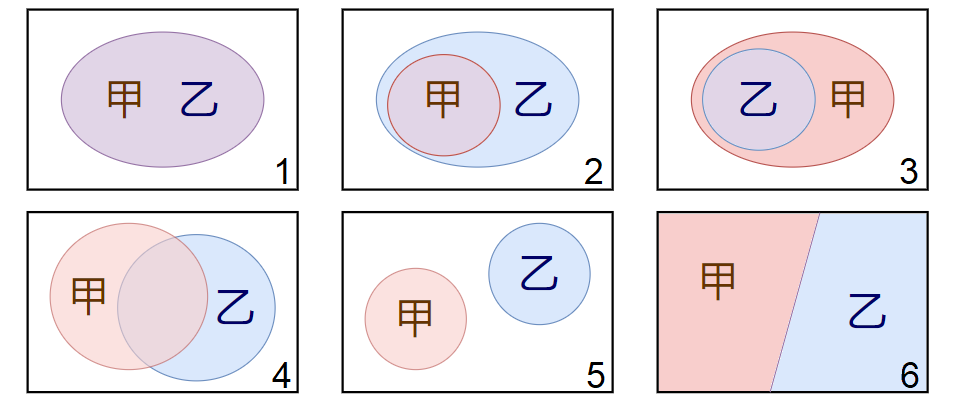
\includegraphics[width=0.75\textwidth]{tu/概念的关系1.png}
    \captionsetup{justification=centering}
    \caption*{1.\texttt{等同关系}，2.\texttt{从属关系}，3.\texttt{包含关系}，\\4.\texttt{交叉关系}，5.\texttt{互斥关系}，6.\texttt{矛盾关系}。}
\end{figure}

为了更好理解，我们可以用\textbf{叠圈图}直观理解集合的关系。

如下图，每个圈表示一个集合\footnote{也可以用其他形状的区域。}，圈内的区域表示属于该集合的元素，圈外的区域表示不属于该集合的元素，也就是该集合（关于全集的）补集。
两个圈重叠的部分就表示同时属于两者的元素的集合，也就是两个集合的交集。而两个圈各自的部分加上重叠的部分，
就是至少属于其中之一的元素的集合，也就是两个集合的并集。

叠圈图可以让我们直接看到集合之间的关系。可以看到，用集合来解释概念，方便得多。

\begin{xt}\label{xt:2-0-20}
    \mbox{} \\ 
    \indent 1. 请用集合解释概念的属加种差定义方法。\\
    \indent 2. 用叠圈图表示“偶数”、“$3$的倍数”、“自然数”之间的关系。\\
    \indent 3. 三个集合$A,B,C$都是集合$\{1,2,3,4,5,6\}$的子集，它们都不是空集，而且构成集合$\{1,2,3,4,5,6\}$的分划。\\
    \indent 3.1. 请写出一个符合条件的$A,B,C$的例子。\\
    \indent 3.2. 符合条件的$A,B,C$一共有几种？
\end{xt}

\section{判断和集合}
理解了概念和集合的关系，我们可以用集合的概念来重新看待判断和命题。

简单的性质判断，只涉及一个概念和一个性质。在对应的命题里，概念是主语，性质是谓语。
我们把主语的概念记为$A$，把谓语的性质记为$b$，那么简单的性质判断可以写成：
$$ A \,\,\mbox{是} \,\,b. $$
如果把$a$看成集合，把用$B$表示所有具有性质$b$的东西的集合。那么，性质判断“$A$是$b$”就是说：
$$A \subseteq B$$
所以，简单的性质判断，就是描述概念的从属关系，也就是集合的子集关系。
判断为真，就是说$A \subseteq B$成立；判断为假，就是说$A \subseteq B$不成立。

\begin{wrapfigure}[5]{r}{0.26\textwidth} %this figure will be at the right
    \vspace{-32pt}
    \flushright
    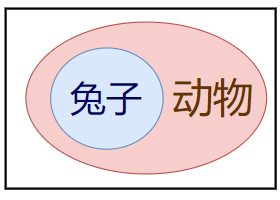
\includegraphics[width=0.24\textwidth]{tu/判断和集合1.png}
    \caption*{\texttt{命题：兔子是动物。}}
\end{wrapfigure}

如果判断的概念$A$是单独概念，那么它对应的子集只有一个元素。我们把这种只含有一个元素的集合称为\textbf{单元集}。

如果把$A$的元素记为$a$，那么$A = \{a\}$。$\{a\} \subseteq B$实际上就是说$a\in B$。

也就是说，判断的概念$A$是单独概念时，我们实际在判断概念是否属于有某个性质的集合。

我们可以给判断的概念$A$加上全称和有称，比如“所有$A$都是$b$”。“所有”的意思是，
概念$A$的范围里所有的元素，都是$b$。于是，“所有”其实只是再次强调了子集关系。

在数学语言里，我们引进表示全称的符号：$\forall$。它读作“任一”、“任何”、“每个”。
全命题：“所有$A$都是$b$”可以记作“$\forall x \in A$，$x \in B$”。它的意思是“$A$中任一元素都是$B$的元素”。
也就是说，$A$是$B$的子集。

如果我们说“有些$A$是$b$”，我们要表达的意思是，$A$的元素里，有些元素是$b$。这些元素构成$A$的子集，但不一定是$A$。
所以，有命题其实表示$A$和$B$相交，交集不是空集。

\begin{figure}[h]
    \vspace{4pt}
    \centering
    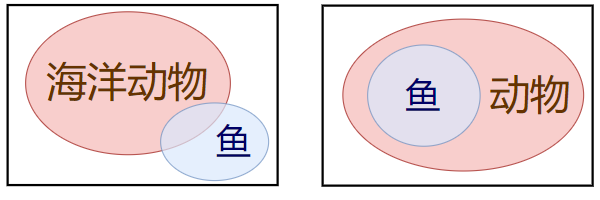
\includegraphics[width=0.5\textwidth]{tu/判断和集合2.png}
    \captionsetup{justification=centering}
    \caption*{\texttt{左：有些鱼是海洋动物，右：所有的鱼都是动物。}}
\end{figure}

在数学语言里，我们引进表示有称的符号：$\exists$。它读作“存在”，“有”，“至少有一个”。
有命题“有些$A$是$b$”可以记作“$\exists x \in A$，$x \in B$”。它的意思是“$A$中至少有一元素是$B$的元素”。
也就是说，$A$和$B$的交集不是空集。

举例来说，“所有偶数都是自然数”可以写作“$\forall x \in \{\mbox{偶数}\}$，$x \in \{\mbox{自然数}\}$”，
换句话说，偶数集是自然数集的子集。
“有些偶数是$3$的倍数”可以写作“$\exists x \in \{\mbox{偶数}\}$，$x \in \{3\mbox{的倍数}\}$”，换句话说，
偶数集和$3$的倍数的集合相交，交集不是空集。

\begin{et}
    用代数的方法，表示加法和乘法的交换律、结合律。
\end{et}

\begin{so}
    加法的交换律：任意两个数相加，交换次序，和不变。把两个数用$a$、$b$表示，加法交换律可以表示成：
    $$ \forall \,\, a, b, \quad a + b = b + a. $$
    
    加法的结合律：任意三个数相加，先把前两个数相加，或者先把后两个数相加，和不变。把三个数用$a$、$b$、$c$表示，加法结合律可以表示成：
    $$ \forall \,\, a, b, c, \quad (a + b) + c = a + (b + c). $$
    
    乘法的交换律：任意两个数相乘，交换次序，积不变。把两个数用$a$、$b$表示，乘法交换律可以表示成：
    $$ \forall \,\, a, b, \quad a \times b = b \times a. $$
    
    乘法的结合律：任意三个数相乘，先把前两个数相乘，或者先把后两个数相乘，积不变。把三个数用$a$、$b$、$c$表示，乘法结合律可以表示成：
    $$ \forall \,\, a, b, c, \quad (a \times b) \times c = a \times (b \times c). $$
\end{so}

复合判断，也可以用集合的方式表达。

联言判断是多个判断的全判断。考虑这样的联言判断：$A$不仅是$b$，也是$c$。
它表达的意思是，$A$不仅包含于性质$b$对应的集合$B$，也包含于性质$c$对应的集合$C$。
$A$的元素同时在$B$、$C$中。换句话说，$A$是$B$、$C$的交集的子集。

一般来说，考虑关于概念$A$的联言判断，它表达的是$A$包含于多个性质对应的集合的交集。
如果把这些性质的集合记为$I$，把每个性质对应的集合记为$B_i$，那么联言判断就是说，
$A$包含于它们的交集，记为：
$$ A \subseteq \bigcap_{i\in I} B_i. $$

或言判断是多个判断的有判断。考虑这样的或言判断：$A$也许$b$，也许$c$。
它表达的意思是，$A$可能包含于性质$b$对应的集合$B$，也可能包含于性质$c$对应的集合$C$。
$A$的元素至少在$B$、$C$中的一个里。换句话说，$A$是$B$、$C$的并集的子集。

一般来说，考虑关于概念$A$的或言判断，它表达的是$A$包含于多个性质对应的集合的并集。
如果把这些性质的集合记为$I$，把每个性质对应的集合记为$B_i$，那么或言判断就是说，
$A$包含于它们的交集，记为：
$$ A \subseteq \bigcup_{i\in I} B_i. $$

\begin{wrapfigure}{r}{0.42\textwidth} %this figure will be at the right
    \vspace{-28pt}
    \flushright
    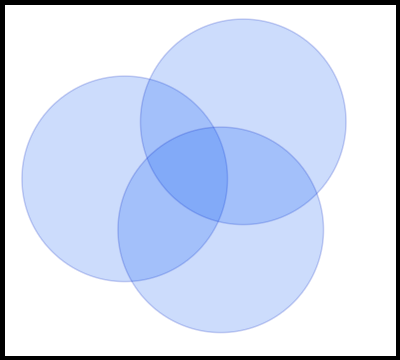
\includegraphics[width=0.4\textwidth]{tu/叠圈图1.png}
\end{wrapfigure}

右图中，每个圈代表一个分支判断对应的集合。联言判断对应着所有圈交叠的区域（颜色最深的部分），而或言判断对应着所有蓝色的区域的总和。

\begin{sk}\label{sk:2-1-1}
     有个理发师，坚持只给那些不给自己理发的人理发。那么，他是否该给自己理发呢？
\end{sk}

\begin{xt}\label{xt:2-1-1}
    \mbox{} \\
    \indent 1. 用代数的方法，表示乘法对加法的分配律。\\
    \indent 2. 用代数的方法，表示乘方的运算法则。\\
    \indent 3. 考虑假言判断：如果$A$是$b$，那么$A$是$c$。设性质$b$、$c$对应的集合是$B$、$C$，集合$A$、$B$、$C$之间有什么关系？\\
    \indent 4. 从集合的角度，解释这句话：“如果全部$A$都是$b$，那么有些$A$是$b$”。
\end{xt}

\section{映射}
我们用\textbf{映射}表示事物之间的对应关系。把一个事物对应到另一个事物，可以理解为事物的变换或对事物进行操作。
因此映射也叫做\textbf{变换}或\textbf{操作}。把数量对应到数量的映射，叫做\textbf{函数}。

\begin{ex}\label{ex:2-2-0}
    \mbox{} \\ 
    \indent 1. 把现有《道德经》各个版本和它的字数对应起来，就是一个映射：
    $$
    \begin{array}{lll}
        \mbox{王弼《老子道德经注》（通行本）} &\longrightarrow &\quad 5162\mbox{字} \\
        \mbox{河上公《道德经章句》} &\longrightarrow &\quad 5201\mbox{字} \\ 
        \mbox{傅奕《道德经古本》} &\longrightarrow &\quad 5450\mbox{字} \\
        \mbox{马王堆帛书甲本} &\longrightarrow &\quad 5344\mbox{字} \\
        \mbox{马王堆帛书乙本} &\longrightarrow &\quad 5342\mbox{字} \\
        \mbox{郭店楚墓本} &\longrightarrow &\quad 2046\mbox{字}
    \end{array}
    $$
    \indent 2. 把事物对应到自己的映射叫做\textbf{恒等映射}或\textbf{等映射}。比如，把每个自然数对应到自己的映射就叫自然数集上的恒等映射，也叫恒等函数。任何非空集合上都有恒等映射。恒等映射的定义域和值域相同。\\
    \indent 3. 把事物对应到同一个对象的映射叫做\textbf{恒映射}或\textbf{常映射}。比如，把任意自然数对应到$0$的映射就是恒映射。
\end{ex}

我们把映射涉及的事物用两个集合记录：\textbf{出发集}和\textbf{到达集}。映射把出发集的一个元素对应到到达集的一个元素。
用变量$x$指代出发集的元素，$x$的取值在出发集里变化时，映射对应的元素也在到达集里变化，可以用变量$y$表示。
一般称$x$为\textbf{自变量}，$y$为\textbf{应变量}。出发集和到达集都是数集的时候，映射就叫做函数。

需要强调的是，映射可以把多个元素对应到同一个元素，但不会把一个元素对应到多个元素。

% 来自 https://commons.wikimedia.org/wiki/File:Function_color_example_3.svg
\begin{figure}[h]
    \vspace{4pt}
    \centering
    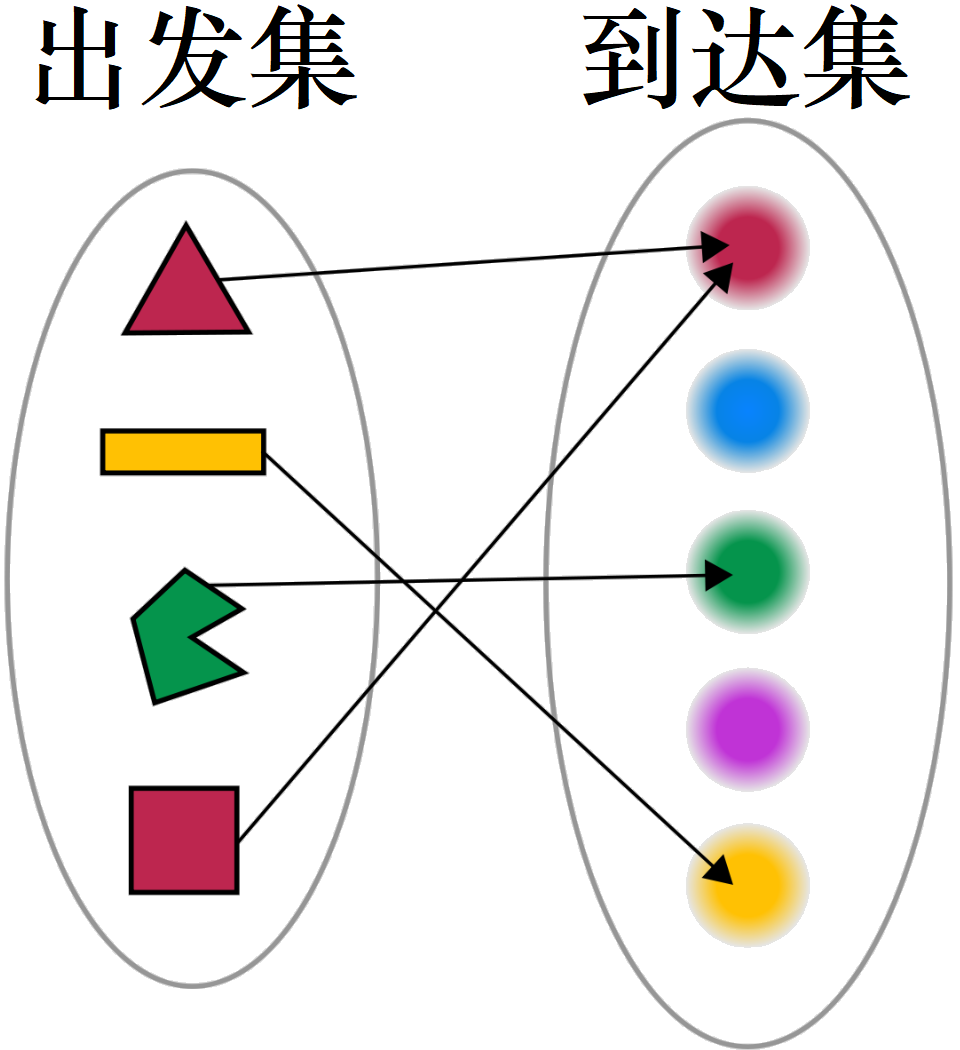
\includegraphics[width=0.5\textwidth]{tu/映射1.png}
    \caption*{\texttt{映射把图形对应到它的颜色}}
\end{figure}

如果把映射记作$f$，那么可以用$y = f(x)$或$f:x\mapsto y$表达“映射把出发集的元素和到达集的元素对应起来”这件事。
对出发集的元素$x$来说，如果映射$f$把它和到达集的元素$y$对应起来，就说$y$是$x$（经过$f$映射）的\textbf{值}，记作$f(x) = y$。

出发集中，某个映射涉及的元素集合称为映射的\textbf{定义域}；
到达集里，某个映射涉及的元素集合则称为映射的\textbf{值域}。定义域是出发集的子集，值域是到达集的子集。

举例来说，映射$f$的定义域是$\{1,2,3,4,5\}$，它把$1,2,3,4,5$分别对应到$6,7,8,7,6$。
那么它的值域是$\{6,7,8\}$。具体来说，$f(2) = 7$，$f(3) = 8$。

% 考虑映射$f$的定义域的子集$S$。$S$中元素经过$f$映射的值，构成值域的子集。
% 我们把它叫做$S$（关于$f$）的\textbf{像集}，简称$S$的\textbf{像}，记作$f(S)$。

% 反之，考虑映射$f$的值域的子集$T$。$T$中元素总是$f$的定义域中元素的值。
% 我们把$f$的定义域里值属于$T$的元素集合起来。这个集合叫做$T$关于$f$的\textbf{原像}。

% 举例来说，映射$f$的定义域是$\{1,2,3,4,5\}$，它把$1,2,3,4,5$分别对应到$6,7,8,7,6$。
% 那么，集合$\{1,2,3,4\}$的像集是$\{6,7,8\}$；集合$\{1,2\}$的像集是$\{6,7\}$。
% 集合$\{7,8\}$的原像是$\{2,3,4\}$；集合$\{6,8\}$的原像是$\{1,3,5\}$。

% 我们约定，空集的像集是空集，空集的原像是空集。

每个一元式都可以用来定义映射。比如，设定定义域是自然数集$\mathbb{N}$后，
代数式$4-0.3x+9x^2+\frac{(1-x+2.69x^4)}{0.5x-1.385}$就可以定义映射：
$$ \forall x\in\mathbb{N}, \quad x \mapsto 4-0.3x+9x^2+\frac{(1-x+2.69x^4)}{0.5x-1.385}. $$
如果把定义域设成另一个集合，比如$\{1,2,3\}$或全体偶数，就定义了另一个映射。

我们知道，每个概念都对应某种集合。如果我们把这个集合作为定义域或者出发集，那么，
确定了定义域后，每个含有变量的简单性质判断就可以定义一个映射。

比如，考虑这样一个命题：“$\{1,2,5,6\}$中的任何数$n$都能被$5$整除”。
我们可以看到，定义域是$\{1,2,5,6\}$，而“$n$能被$5$整除”就可以定义以下的映射：
$$ \forall n\in \{1,2,5,6\} , \quad n \mapsto n\,\mbox{能被}\,5\,\mbox{整除。} $$
这个映射从简单判断的主语出发。主语的概念对应集合$\{1,2,5,6\}$。

对集合中每个单独的元素$n$，
“$n$能被$5$整除”这个判断要么是真的，要么是假的。因此，如何我们考虑集合$\{\mbox{真}, \mbox{假}\}$，
那么这个集合就是上面的映射的到达集，因为对每个$n$来说，“$n$能被$5$整除”这个判断要么是真的，要么是假的。
而它的值域就是集合$\{\mbox{真}, \mbox{假}\}$的子集。

“真”、“假”就是命题的真值，所以我们一般把这个集合称为\textbf{真值集}或者\textbf{二元集}。
很多时候，我们也会用$0$表示“假”，$1$表示“真”\footnote{也有的时候会反过来。}。

\begin{sk}\label{sk:2-2-0}
    \mbox{} \\
    \indent 1. 全判断$\forall x \in A, \, P(x)$和映射$x \mapsto P(x)$之间存在什么关系？\\
\end{sk}

\begin{xt}\label{xt:2-2-0}
    \mbox{} \\
    \indent 1. 映射$f$的定义域是$\{1,2,3\}$，值域是$\{4,5\}$。\\
    \indent 1.1. 写出一个满足条件的映射$f$。\\
    \indent 1.2. 你能写出几个满足条件的映射$f$？\\
    \indent 2. 判断以下说法是否正确。\\
    \indent 2.1. 到达集中的元素，总是映射的结果。\\
    \indent 2.2. 出发集中的元素经过映射的值，总在映射的值域中。%\\
    % \indent 2.3. 映射的定义域的元素构成的集合，其像集的原像总是自己。\\
    % \indent 2.4. 映射的值域的元素构成的集合，其原像的像集总是自己。\\
    % \indent 3. 考虑以下映射和集合，给出相应的像集或原像。\\
    % \indent 3.1. 映射$f$把正整数对应到它的$3$倍数。比如：$f(1) = 3$，$f(2) = 6$，等等。求集合$\{21, 39, 87\}$的像集和原像。\\
    % \indent 3.2. 映射$g$把月份对应到它的天数（不考虑闰年）。比如一月的值是$31$，二月的值是$28$，等等。求集合$\{30\}$的原像。\\
    % \indent 3.3. 映射$h$把汉字对应到它的笔画数。比如“数”的值是$13$，“学”的值是$8$，等等。设集合$S$是$\{1,2\}$的原像，请写出它的十个元素。 % 一二七八九 十人入丁乃 儿了几刀刁 力匕卜厂又
\end{xt}

\chapter{判断和命题}  % 初中第二册第1章

数学自古以来也称为算学，我们已经学习了不少关于计算的方法和知识。不过，数学对现代社会产生重要影响，不仅仅由于计算，还在于数学给我们提供了思考问题的精确方法。

上一本书中，我们学习了代数，也就是用字母等符号代替数字来思考的方法。通过用字母代替具体的数字，我们从繁多的运算和关系中抽出我们想讨论的性质和问题。我们说，考虑抽象的概念、性质和问题，是数学的根本任务。具体如何处理这些概念、思考这些问题呢？千百年来，数学家积累了一套思考的经验方法，总结出可行的规律，称为\textbf{思理}。掌握了思理，我们才能正确地思考，正确地处理抽象的概念和性质，正确地解决问题。我们已经接触过一些基本的思理。下面就让我们开始进一步的学习。

\section{充分条件和必要条件}
我们已经学过判断：\textbf{判断}，是对事物情况表达肯定或否定的态度。判断包括简单判断和复合判断。
简单判断包括性质判断和关系判断。性质判断包括全判断、有判断和单判断；复合判断包括联言判断、或言判断、选言判断和假言判断。

假言判断是关于条件的判断，它涉及两个称为\textbf{前件}和\textbf{后件}的判断，并判断前件是后件成立的条件。
假言判断并不对前件或后件做判断，只对两者的条件关系做判断，而条件关系又分为两种：\textbf{充分条件}和\textbf{必要条件}。

充分条件假言判断想说的是：前件为真的时候，后件也为真。比如：人如果不吃东西，就会饿。
这个例子里，前件是“人不吃东西”，后件是“人会饿”。前件真的时候，后件也是真的，这说明充分条件关系是真的。
我们说，前件是后件的充分条件。这个例子里，“人不吃东西”是“人会饿”的充分条件。

\begin{et}\label{et:2-0-0}
    \mbox{}\\
    \indent “你要是考了满分，母猪都会上树了！”\\
    \indent 1. 这句话里，“你考了满分”和“母猪会上树”是什么关系？\\
    \indent 2. “你”如果没考满分，这个关系还成立吗？这时“母猪会上树”和“母猪不会上树”对这个判断有什么影响？
\end{et}

充分条件判断的真值表为：
\begin{center}
    \begin{tabular}{ p{3em}<{\centering} p{3em}<{\centering} p{8em}<{\centering} }
        \rowcolor{gd} $p$ & $q$ & 如果$p$，那么$q$ \\ [0.5ex] 
        \noalign{{\color{white}\hrule height 2pt}} % \hline\hline
        \rowcolor{gl} 真 & 真 & 真  \\  
        \noalign{{\color{white}\hrule height 2pt}}% \hline
        \rowcolor{gd} 真 & 假 & 假  \\
        \noalign{{\color{white}\hrule height 2pt}}% \hline
        \rowcolor{gl} 假 & 真 & 真 \\  
        \noalign{{\color{white}\hrule height 2pt}}% \hline
        \rowcolor{gd} 假 & 假 & 真 \\
    \end{tabular}
\end{center}

必要条件假言判断想说的是：前件为假的时候，后件也为假。比如：人只有识字了，才能读书。
这个例子里，前件是“识字”，后件是“能读书”。不识字的人，不能读书。前件假的时候，后件也是假的，这说明必要条件关系是真的。
我们说，前件是后件的必要条件。这个例子里，“识字”是“能读书”的必要条件。

\begin{et}\label{et:2-0-1}
    \mbox{}\\
    \indent “只有到了晚上，才能看见满天的星星。”\\
    \indent 1. 这句话里，“到了晚上”和“看见星星”是什么关系？\\
    \indent 2. 有时，到了晚上也看不见星星。是否说明这个判断不成立呢？
\end{et}

必要条件判断的真值表为：
\begin{center}
    \begin{tabular}{ p{3em}<{\centering} p{3em}<{\centering} p{8em}<{\centering} }
        \rowcolor{gd} $p$ & $q$ & 只有$p$，才有$q$ \\ [0.5ex] 
        \noalign{{\color{white}\hrule height 2pt}} % \hline\hline
        \rowcolor{gl} 真 & 真 & 真  \\  
        \noalign{{\color{white}\hrule height 2pt}}% \hline
        \rowcolor{gd} 真 & 假 & 真  \\
        \noalign{{\color{white}\hrule height 2pt}}% \hline
        \rowcolor{gl} 假 & 真 & 假 \\  
        \noalign{{\color{white}\hrule height 2pt}}% \hline
        \rowcolor{gd} 假 & 假 & 真 \\
    \end{tabular}
\end{center}

如果前件既是后件的充分条件，也是后件的必要条件，就说前件是后件的\textbf{充要条件}。
充要条件一般用“当且仅当”句式来表达。比如：“李四年纪比张三大，当且仅当张三年纪比李四小。”

充要条件假言判断可以看成充分条件假言判断和必要条件假言判断的联言判断。因此，充要条件判断的真值，
可以通过充分条件判断的真值和必要条件判断的真值得到：
\begin{center}
    \begin{tabular}{ p{3em}<{\centering} p{3em}<{\centering} p{7em}<{\centering} p{7em}<{\centering} p{7em}<{\centering} }
        \rowcolor{gd} $p$ & $q$ & 如果$p$，那么$q$ & 只有$p$，才有$q$ & $p$，当且仅当$q$ \\ [0.5ex] 
        \noalign{{\color{white}\hrule height 2pt}} % \hline\hline
        \rowcolor{gl} 真 & 真 & 真 & 真 & 真 \\  
        \noalign{{\color{white}\hrule height 2pt}}% \hline
        \rowcolor{gd} 真 & 假 & 假 & 真 & 假 \\
        \noalign{{\color{white}\hrule height 2pt}}% \hline
        \rowcolor{gl} 假 & 真 & 真 & 假 & 假 \\  
        \noalign{{\color{white}\hrule height 2pt}}% \hline
        \rowcolor{gd} 假 & 假 & 真 & 真 & 真\\
    \end{tabular}
\end{center}
可以看到，前件和后件都为真、都为假的时候，充要条件判断为真。前件和后件一真一假的时候，充要条件判断为假。

\begin{sk}\label{sk:2-0-0} 前件和后件互换位置，充要条件判断是否会变化？这说明了什么？
\end{sk}

和其他判断一样，我们可以从集合的角度来看假言判断。

比如说，在充分条件假言判断“如果$X$是$a$，那么$X$是$b$”中，
我们记性质$a$、$b$对应的集合为$A$、$B$。这个判断的意思是$A$的元素总在$B$里。换句话说，$A$是$B$的子集\footnote{这里我们要求前后件的主语一致，也就是说，$A$、$B$都包含于同一个母集$X$。下同。}。

又比如，在必要条件假言判断“只有$X$是$a$，$X$才是$b$”中，
我们记性质$a$、$b$对应的集合为$A$、$B$。这个判断的意思要成为$B$的元素，首先得是$A$的元素，即$B$的元素总在$A$里。换句话说，$B$是$A$的子集。

而充要条件判断“$X$是$a$，当且仅当$X$是$b$”，同时是充分条件判断和必要条件判断，也就是说，$A$和$B$互为子集，因此，充要条件判断就是说它们对应的集合相同。

\section{命题的否定}
\textbf{命题}就是包含判断的语句。\textbf{命题的否定}，是一个真假和原来的命题恰好相反的命题。
只要原来的命题是真的，它就是假的。
只要原来的命题是假的，它就是真的。
比如，命题“$4$是偶数”的否定是“$4$不是偶数”。

对生活中具体的命题来说，命题的否定可能有多种多样的形式，和使用的语言、文体、措辞都有关系。
数学上，为了方便，我们把命题$p$的否定记为“非$p$”。

判断一个命题是不是命题的否定，可以通过真值表。如果在每种情况下，命题$q$的真值和命题$p$的真值都相反，
那么$q$就是$p$的否定。

对简单性质判断构成的命题来说，命题的否定取决于全称、有称还是单称。

单命题的否定就是它的反命题。
比如：“小明不是校篮球队的队员”的否定是“小明是校篮球队的队员”，“$4$是偶数”的否定是“$4$不是偶数”。

全命题的否定是它的有反命题，有命题的否定是它的全反命题。
比如：“四年级所有的学生都参加了校运会”的否定是“有些四年级的学生没有参加校运会”，
“有些树会落叶”的否定是“所有的树都不落叶”。

为了方便，我们把否定记为$\neg$，比如$p$的否定记为$\neg p$。于是，以上的结论可以写成：
\begin{align*}
    \neg  (\forall a\in A, \,\,\, P(a)) &= (\exists a\in A, \,\,\, \neg P(a)),  \\
    \neg  (\exists a\in A, \,\,\, P(a)) &= (\forall a\in A, \,\,\, \neg P(a)). 
\end{align*}

对复合命题，命题的否定涉及到构成复合命题的各个部分。

观察以下真值表，你有什么发现？
\begin{center}
    \begin{tabular}{ p{2em}<{\centering} p{2em}<{\centering} p{4em}<{\centering} p{4em}<{\centering} p{6em}<{\centering} p{6em}<{\centering} }
        \rowcolor{gd} $p$ & $q$ & $p$并且$q$ & $p$或者$q$ & 非$p$并且非$q$ & 非$p$或者非$q$\\ [0.5ex] 
        \noalign{{\color{white}\hrule height 2pt}} % \hline\hline
        \rowcolor{gl} 真 & 真 & 真 & 真 & 假 & 假 \\  
        \noalign{{\color{white}\hrule height 2pt}}% \hline
        \rowcolor{gd} 真 & 假 & 假 & 真 & 假 & 真\\
        \noalign{{\color{white}\hrule height 2pt}}% \hline
        \rowcolor{gl} 假 & 真 & 假 & 真 & 假 & 真\\  
        \noalign{{\color{white}\hrule height 2pt}}% \hline
        \rowcolor{gd} 假 & 假 & 假 & 假 & 真 & 真\\
    \end{tabular}
\end{center}
我们发现，命题$p$和$q$取遍所有可能的情况时，联言命题“$p$并且$q$”和或言命题“非$p$或者非$q$”的真假刚好相反。
同样，或言命题“$p$或者$q$”和联言命题“非$p$并且非$q$”的真假也刚好相反。因此，“$p$并且$q$”的否定是“非$p$或者非$q$”。
“$p$或者$q$”的否定“非$p$并且非$q$”

联言命题的否定，是它各个分支的否定的或言命题；或言命题的否定，是它各个分支的否定的联言命题。

为了方便，我们把“$p$并且$q$”记为$p\wedge q$，把“$p$或者$q$”记为$p\vee q$。于是，上面的规则可以简单记为：
$$ \neg (p \wedge q) = (\neg p) \vee (\neg q), \quad \neg (p \vee q) = (\neg p) \wedge (\neg q). $$

观察以下真值表，你有什么发现？
\begin{center}
    \begin{tabular}{ p{2em}<{\centering} p{2em}<{\centering} p{4em}<{\centering} p{5em}<{\centering} p{5em}<{\centering} p{6em}<{\centering} }
        \rowcolor{gd} $p$ & $q$ & 若$p$则$q$ & 若$p$则非$q$ & $p$而且非$q$ & 若非$p$则非$q$\\ [0.5ex] 
        \noalign{{\color{white}\hrule height 2pt}} % \hline\hline
        \rowcolor{gl} 真 & 真 & 真 & 假 & 假 & 真 \\  
        \noalign{{\color{white}\hrule height 2pt}}% \hline
        \rowcolor{gd} 真 & 假 & 假 & 真 & 真 & 真\\
        \noalign{{\color{white}\hrule height 2pt}}% \hline
        \rowcolor{gl} 假 & 真 & 真 & 真 & 假 & 假\\  
        \noalign{{\color{white}\hrule height 2pt}}% \hline
        \rowcolor{gd} 假 & 假 & 真 & 真 & 假 & 真\\
    \end{tabular}
\end{center}
我们发现，命题$p$和$q$取遍所有可能的情况时，充分条件假言命题“若$p$则$q$”的否定不是“若$p$则非$q$”，也不是“若非$p$则非$q$”，
而是“$p$而且非$q$”。为了方便，我们把“若$p$则$q$”记为$p \Rightarrow q$，于是：
$$ \neg (p \Rightarrow q) = p \wedge (\neg q).$$

观察以下真值表，你有什么发现？
\begin{center}
    \begin{tabular}{ p{3em}<{\centering} p{3em}<{\centering} p{7em}<{\centering} p{5em}<{\centering} }
        \rowcolor{gd} $p$ & $q$ & 只有$p$，才有$q$ & $q$而且非$p$\\ [0.5ex] 
        \noalign{{\color{white}\hrule height 2pt}} % \hline\hline
        \rowcolor{gl} 真 & 真 & 真 & 假 \\  
        \noalign{{\color{white}\hrule height 2pt}}% \hline
        \rowcolor{gd} 真 & 假 & 真 & 假 \\
        \noalign{{\color{white}\hrule height 2pt}}% \hline
        \rowcolor{gl} 假 & 真 & 假 & 真 \\  
        \noalign{{\color{white}\hrule height 2pt}}% \hline
        \rowcolor{gd} 假 & 假 & 真 & 假 \\
    \end{tabular}
\end{center}
我们发现，命题$p$和$q$取遍所有可能的情况时，必要条件假言命题“只有$p$，才有$q$”的否定是“$q$而且非$p$”。
为了方便，我们把“只有$p$，才有$q$”记为$p \Leftarrow q$，于是：
$$ \neg (p \Leftarrow q) = (\neg p) \wedge q.$$

观察以下真值表，你有什么发现？
\begin{center}
    \begin{tabular}{ p{3em}<{\centering} p{3em}<{\centering} p{7em}<{\centering} p{7em}<{\centering} }
        \rowcolor{gd} $p$ & $q$ & $p$当且仅当$q$ & 要么$p$，要么$q$\\ [0.5ex] 
        \noalign{{\color{white}\hrule height 2pt}} % \hline\hline
        \rowcolor{gl} 真 & 真 & 真 & 假 \\  
        \noalign{{\color{white}\hrule height 2pt}}% \hline
        \rowcolor{gd} 真 & 假 & 真 & 假 \\
        \noalign{{\color{white}\hrule height 2pt}}% \hline
        \rowcolor{gl} 假 & 真 & 假 & 真 \\  
        \noalign{{\color{white}\hrule height 2pt}}% \hline
        \rowcolor{gd} 假 & 假 & 真 & 假 \\
    \end{tabular}
\end{center}
我们发现，命题$p$和$q$取遍所有可能的情况时，充要条件假言命题“$p$当且仅当$q$”的否定是选言命题“要么$p$，要么$q$”。
为了方便，我们把“$p$当且仅当$q$”记为$p \Leftrightarrow q$，把“要么$p$，要么$q$”记为$p \oplus q$。于是：
$$ \neg (p \Leftrightarrow q) = p \oplus q.$$

\begin{sk}\label{sk:2-1-0}
    命题“要么$p$，要么非$q$”的否定是什么？
\end{sk}

\begin{xt}\label{xt:2-1-0}
    以下例子中，后面的命题是前面的命题的否定吗？\\
    \indent 1. “如果不下雨，我就把印章送过去”和“如果下雨，我就把印章送过去”。\\
    \indent 2. “如果$n$是$3$的倍数，那么$m$是$7$的倍数”和“$n$是$3$的倍数，而且$m$不是$7$的倍数”。\\
    \indent 3. “如果旅馆不提供早餐，那么有些队员不愿意参加秋季合宿训练计划”和“旅馆不提供早餐，而且有些队员愿意参加秋季合宿训练计划”。
    % 4. “线段$AB$上有些点既是中线上的点，也是垂直平分线上的点”和“线段$AB$上所有点既不是中线上的点，也不是垂直平分线上的点”。
\end{xt}

\section{逆命题、否命题和逆否命题}
前面提到，复合命题的否定涉及它的组成部分。我们已经研究了联言命题、或言命题和假言命题的否定。
另一个涉及到复合命题各个组成部分的概念是逆命题和否命题。

给定两个假言命题，如果第一个命题的前件和后件分别是第二个命题的后件和前件，就说两者\textbf{互为逆命题}。
换句话说，把假言命题中的前件和后件互换，就得到它的\textbf{逆命题}。比如，给定假言命题：
“如果$n$是偶数，那么$m$是奇数”的逆命题是“如果$m$是奇数，那么$n$是偶数”。

一个命题是真的，它的逆命题不一定是真的。比如，已知两个角$\angle A$和$\angle B$，
命题“如果$\angle A$和$\angle B$是对顶角，那么它们相等”是真的；
但它的逆命题：“如果$\angle A$和$\angle B$相等，那么它们是对顶角”是假的。
反之，一个命题的逆命题是真的，它自身也不一定是真的。

给定两个假言命题，如果第一个命题的前件和后件分别是第二个命题的前件和后件的否定，就说两者\textbf{互为否命题}。
换句话说，把假言命题中的前件和后件换成它们各自的否定，就得到它的\textbf{否命题}。
比如，假言命题“如果$n$是$6$的倍数，那么$n$是$3$的倍数”的否命题是“如果$n$不是$6$的倍数，那么$n$不是$3$的倍数”。

否命题和命题的否定不是同一个概念。一个命题是真的，它的否定必然是假的，但它的否命题不一定是假的。
一个命题是假的，它的否定必然是真的，但它的否命题不一定是真的。
比如，已知两个角$\angle A$和$\angle B$，“如果$\angle A$和$\angle B$是对顶角，那么它们相等”是真的，
它的否命题“如果$\angle A$和$\angle B$不相等，那么它们不是对顶角”也是真的。
但是，命题“如果$n$是$6$的倍数，那么$n$是$3$的倍数”是真的，
它的否命题“如果$n$不是$6$的倍数，那么$n$不是$3$的倍数”却是假的。

假言命题的否命题的逆命题，就是先把前件和后件中的判断都改成否判断，再把前件和后件互换。
要注意的是，假言命题的否命题的逆命题，和假言命题的逆命题的否命题是一样的。
因为前后件互换和同时把前后件变成否判断这两个操作互相并不妨碍。这样得到的命题称为原来的假言命题的\textbf{逆否命题}。
比如，“如果$n$是$6$的倍数，那么$n$是$3$的倍数”的逆否命题是
“如果$n$不是$3$的倍数，那么$n$不是$6$的倍数”。

不难验证，一个命题的逆命题的逆命题是它自己，一个命题的否命题的否命题是它自己，
一个命题的逆否命题的逆否命题，也是它自己。

观察以下真值表，你有什么发现？
\begin{center}
    \begin{tabular}{ p{3em}<{\centering} p{3em}<{\centering} p{4em}<{\centering} p{4em}<{\centering} p{6em}<{\centering} p{6em}<{\centering} }
        \rowcolor{gd} $p$ & $q$ & $p\Rightarrow q$ & $q\Rightarrow p$ & $\neg p\Rightarrow \neg q$ & $\neg q\Rightarrow \neg p$ \\ [0.5ex] 
        \noalign{{\color{white}\hrule height 2pt}} % \hline\hline
        \rowcolor{gl} 真 & 真 & 真 & 真 & 真 & 真 \\  
        \noalign{{\color{white}\hrule height 2pt}}% \hline
        \rowcolor{gd} 真 & 假 & 假 & 真 & 真 & 假\\
        \noalign{{\color{white}\hrule height 2pt}}% \hline
        \rowcolor{gl} 假 & 真 & 真 & 假 & 假 & 真\\  
        \noalign{{\color{white}\hrule height 2pt}}% \hline
        \rowcolor{gd} 假 & 假 & 真 & 真 & 真 & 真\\
    \end{tabular}
\end{center}
我们发现，命题$p$和$q$取遍所有可能的情况时，充分条件假言命题“$p\Rightarrow q$”和它的逆否命题“$\neg q\Rightarrow \neg p$”的真假值完全一样。
于是：
$$ p \Rightarrow q = (\neg q) \Rightarrow (\neg p). $$
另一方面，命题“$p\Rightarrow q$”的逆命题“$q\Rightarrow p$”和“$p\Rightarrow q$”的否命题“$\neg p\Rightarrow \neg q$”的真假值也完全一样。
这是因为“$q\Rightarrow p$”的逆否命题就是“$\neg p\Rightarrow \neg q$”。

观察以下真值表，你有什么发现？
\begin{center}
    \begin{tabular}{ p{3em}<{\centering} p{3em}<{\centering} p{4em}<{\centering} p{4em}<{\centering} p{6em}<{\centering} p{6em}<{\centering} }
        \rowcolor{gd} $p$ & $q$ & $p\Leftarrow q$ & $q\Leftarrow p$ & $\neg p\Leftarrow \neg q$ & $\neg q\Leftarrow \neg p$ \\ [0.5ex] 
        \noalign{{\color{white}\hrule height 2pt}} % \hline\hline
        \rowcolor{gl} 真 & 真 & 真 & 真 & 真 & 真 \\  
        \noalign{{\color{white}\hrule height 2pt}}% \hline
        \rowcolor{gd} 真 & 假 & 假 & 真 & 真 & 假\\
        \noalign{{\color{white}\hrule height 2pt}}% \hline
        \rowcolor{gl} 假 & 真 & 真 & 假 & 假 & 真\\  
        \noalign{{\color{white}\hrule height 2pt}}% \hline
        \rowcolor{gd} 假 & 假 & 真 & 真 & 真 & 真\\
    \end{tabular}
\end{center}
我们发现，命题$p$和$q$取遍所有可能的情况时，必要条件假言命题“$p\Leftarrow q$”
和它的逆否命题“$\neg q\Leftarrow \neg p$”的真假值完全一样。
于是：
$$ p \Leftarrow q = (\neg q) \Leftarrow (\neg p). $$
另一方面，我们还可以注意到，命题$p$和$q$取遍所有可能的情况时，“$q\Rightarrow p$”的真假值和“$p\Leftarrow q$”
完全一样。这说明，充分条件假言命题“$p\Rightarrow q$”的逆命题就是“$p\Leftarrow q$”。

观察以下真值表，你有什么发现？
\begin{center}
    \begin{tabular}{ p{3em}<{\centering} p{3em}<{\centering} p{4em}<{\centering} p{4em}<{\centering} p{6em}<{\centering} p{6em}<{\centering} }
        \rowcolor{gd} $p$ & $q$ & $p \Leftrightarrow q$  & $q \Leftrightarrow p$  & $\neg p \Leftrightarrow\neg q$ & $\neg q \Leftrightarrow \neg p$ \\ [0.5ex] 
        \noalign{{\color{white}\hrule height 2pt}} % \hline\hline
        \rowcolor{gl} 真 & 真 & 真 & 真 & 真 & 真 \\  
        \noalign{{\color{white}\hrule height 2pt}}% \hline
        \rowcolor{gd} 真 & 假 & 假 & 假 & 假 & 假 \\
        \noalign{{\color{white}\hrule height 2pt}}% \hline
        \rowcolor{gl} 假 & 真 & 假 & 假 & 假 & 假 \\  
        \noalign{{\color{white}\hrule height 2pt}}% \hline
        \rowcolor{gd} 假 & 假 & 真 & 真 & 真 & 真 \\
    \end{tabular}
\end{center}
我们发现，命题$p$和$q$取遍所有可能的情况时，充要条件假言命题“$p \Leftrightarrow q$”
和它的逆命题、否命题、逆否命题的真假值完全一样。
于是：
$$ p \Leftrightarrow q = q \Leftrightarrow p = (\neg p) \Leftarrow (\neg q) = (\neg q) \Leftarrow (\neg p). $$

\begin{sk}\label{sk:2-2-1}
    \mbox{} \\
    1. 给定一个充分条件假言命题，分别写出它的否定、它的逆命题的否定、它的否命题的否定和它的逆否命题的否定。
    这些命题之间有什么关系？\\
    2. 观察以下关系图。图中的关系是否正确？如何验证？
\end{sk}

\begin{tikzpicture}[
    node distance=3cm and 4cm,  % 水平和垂直间距
    every node/.style={
        draw, 
        rectangle, 
        minimum width=2.5cm, 
        minimum height=0.8cm, 
        align=center,
        font=\small
    },
    label/.style={
        align=center,
        font=\small,
        draw=none % 不绘制边框
    }
]

% 定义四个命题节点
\node (original) {若\(p\)，则\(q\)};
\node [below right= of original] (inverse_negation) {若\(\neg q\)，则\(\neg p\)};

\node [right= of original] (inverse) {若\(q\)，则\(p\)};
\node [below= of original] (negation) {若\(\neg p\)，则\(\neg q\)};

% 在节点下方添加说明性例子
\node [label,above=-0.2em of original, draw=none] {原命题};
\node [label,below=-0.2em of inverse_negation, draw=none] {逆否命题};
\node [label,above=-0.2em of inverse, draw=none] {逆命题};
\node [label,below=-0.2em of negation, draw=none] {否命题};

% 绘制横向箭头
\draw[draw=red,<->] (original.east) -- node[label,above=-0.2em] {互逆} (inverse.west);
\draw[draw=red,<->] (negation.east) -- node[label,below=-0.2em] {互逆} (inverse_negation.west);

% 绘制竖向箭头
\draw[draw=blue,<->] (original.south) -- node[label,left=-1.3em] {互否} (negation.north);
\draw[draw=blue,<->] (inverse.south) -- node[label,right=-1.3em] {互否} (inverse_negation.north);

% 绘制对角线双向箭头（保持文字正放）
\draw[draw=orange,<->] (original.south east) to[out=-37,in=143] 
    node[label,midway,sloped=false] {互\phantom{安安安安安安.}\\为\phantom{安安}\\\phantom{安安}逆\\\phantom{.安安安安安安}否} 
    (inverse_negation.north west);

\draw[draw=orange,<->] (inverse.south west) to[out=-143,in=37] 
    node[label,midway,sloped=false] {\phantom{安安安安安安.}否\\\phantom{安安}逆\\为\phantom{安安}\\互\phantom{.安安安安安安}} 
    (negation.north east);

\end{tikzpicture}

\begin{xt}\label{xt:2-2-1}
    \mbox{} \\
    \indent 1. 写出以下命题的逆命题、否命题和逆否命题。\\
    \indent 1.1.  如果我无法完成这套体操动作，你也无法完成。\\
    \indent 1.2. 如果既约分数的分母是偶数，那么它的分子是奇数。\\
    \indent 1.3. 如果有些人不能按时完成工作，那么所有人都会受到惩罚。\\
    \indent 2. 证明：必要条件假言命题的逆命题是充分条件假言命题。
\end{xt}

\chapter{从推理到证明}  % 初中第二册第2章

我们知道，判断（命题）之间在真假方面是有联系的。利用其中的规律，我们可以通过已经知道是真的判断，得知另一些判断的真假。这种思考称为\textbf{推理}。推理过程中，已经知道真假的判断，叫做\textbf{前提}；通过思考得知真假的判断，称为\textbf{结论}。

语言形式上，日常语言中的推理一般用“因为……所以……”、“……，因此……”、“由于……，从而……”等句式来表示。
前提一般写在结论前面。

有些推理是符合客观现实的，我们通过总结客观事物的性质，可以验证它们是有效的推理。另外一些推理不符合
客观事实，我们可以验证它们是无效的推理。哪些推理方式是有效的呢？这是一个非常关键的问题。在千百年的社会发展中，人们逐渐总结出一系列正确的推理方式。学会了正确的推理方式，才能得到正确的结论，正确地看待问题、解决问题。

推理是数学和很多学科研究中常见的内容。对数学来说，推理和计算是两种主要的思维形式。数学中的推理形式比日常语言中的推理更复杂，因此要用专门的符号来表示。

\section{换质法}

最简单的推理，是从一个简单判断到另一个简单判断的推理。我们称这种推理为\textbf{直接推理}。
下面我们来看两种直接推理方式。

\begin{et}\label{et:2b-0-0} 
    以下的例子中，前后两句话有什么关联？\\
    \indent 1. 有的哺乳动物是非素食动物。有的哺乳动物不是素食动物。\\
    \indent 2. 所有个位是$3$的数都不是偶数。所有个位是$3$的数都是奇数。\\
    \indent 3. 这盒牛奶不是变质的。这盒牛奶是没变质的。
\end{et}
以上每个例子中，前一句话和后一句话的区别在于：后一句话把前一句话的断语变成了与它矛盾的概念，然后把判断变成了对应的否判断。
比如，第三个例子中，后一句把“变质的”改成了矛盾的概念：“没变质的”，然后把否定句改成了肯定句。

我们发现，这种方法不会改变判断的真假。把判断改成否判断，同时把事物的性质改成矛盾的概念，判断的真假不变。
因此，把一个判断作为前提，把如上改变后的判断作为结论，就得到一个有效的推理。我们一般用“因为……所以……”、“……，因此……”等句式
描述推理。比如，对第三个例子，我们可以这么描述：
\begin{quotation}
    因为这盒牛奶不是变质的，所以这盒牛奶是没变质的。
\end{quotation}

我们把这种推理方法称为\textbf{换质法}。“质”指“肯定句”和“否定句”这两种形式，“换质”指从肯定换为否定或者从否定换为肯定。
\begin{xt}\label{xt:2b-0-0}
    \mbox{} \\
    以下推理是不是有效的推理？为什么？\\
    \indent 1. 因为蚂蚁不是植物，所以蚂蚁是动物。 \\
    \indent 2. 因为这盒牛奶不是脱脂的，所以这盒牛奶是全脂的。 \\
    \indent 3. 因为有的条款不是不可逆的，所以有的条款是可逆的。 \\
    \indent 4. 因为有的董事会成员不反对转型方案，所以有的董事会成员反对不转型方案。
\end{xt}

\section{换位法}
\begin{et}\label{et:2b-1-0} 
    以下的例子中，前后两句话有什么关联？\\
    \indent 1. 有的物理学家是共产主义者。有的共产主义者是物理学家。\\
    \indent 2. 所有的西瓜都是水果。所有的水果都是西瓜。\\
    \indent 3. 陈家洛是红花会的总舵主。红花会的总舵主是陈家洛。
\end{et}
以上每个例子中，前一句话和后一句话的区别在于：后一句话把前一句话的断语变成了主语，然后把主语变成了对应的断语。比如，第二个例子中，后一句把“水果”改成了主语，把“西瓜”改成了宾语。我们把这种操作称为\textbf{换位法}，即交换了判断的主语和断语的位置。

换位法是否改变了判断的真假？

第一个例子中，我们可以确信，只要第一句是真的，那么第二句就是真的。
有的物理学家是共产主义者，比如物理学家奥本海默是共产主义者，那么奥本海默这个共产主义者也的确是物理学家，于是，有的共产主义者是物理学家。

第二个例子中，“所有的西瓜是水果”是真的，但“所有的水果是西瓜”是假的。比如苹果就不是西瓜。

第三个例子中，如果陈家洛是红花会的总舵主，那么红花会的总舵主是不是陈家洛呢？如果红花会的总舵主只有一个，那么他就是陈家洛。如果红花会的总舵主不止一个，那么就不能说“红花会的总舵主是陈家洛”。

我们发现，换位法不总是有效的推理。什么时候，换位法有效呢？从前面的例子看出，换位法无效，总是因为前提里我们并没有在讨论某个概念的全体，在结论里我们却在讨论它的全体。

比如，第二个例子里，前提“所有的西瓜是水果”中讨论了所有的西瓜，但并没有涉及水果这个概念的全体。
我们讨论这个判断的真假时，不需要检查每个水果。可到了结论里，我们却要讨论所有的水果。同样的，第三个例子里，我们讨论“陈家洛是红花会的总舵主”时，并没有涉及所有的红花会总舵主，只讨论陈家洛是不是总舵主。其他总舵主，如果有的话，并不在讨论范围内。而到了结论里，我们却要讨论“红花会的总舵主”全体了。

所以，换位法需要再加一条规则才是有效的推理：\textbf{前提中讨论的概念如果不涉及它的全体，结论中也不能涉及它的全体。}

我们把“概念涉及它的全体”称为概念\textbf{周延}，把“概念不涉及它的全体”称为概念\textbf{不周延}。换位法缺的规则可以复述为：\textbf{前提中讨论的概念如果不周延，它在结论中也不周延。}

举例来说，前提“有的水果不是西瓜”换位到结论“有的西瓜不是水果”是无效的推理，因为前提中
“水果”不周延；而结论中，为了判断“不是水果”，我们需要检查所有的水果，结论中的“水果”周延。

对于主语来说，周延和全判断是一致的，不周延和有判断是一致的。全判断的主语是周延的，有判断的主语是不周延的。

对于断语来说，否定后接的断语总是周延的：为了否定一个性质，我们需要检查这个性质所有的个体。肯定后接的断语总是不周延的：我们只需要对主语涉及的概念进行检查就可以了。比如，要判断“有的水果是西瓜”，我们只需要找一个是西瓜的水果就可以了；而要判断“有的水果不是西瓜”，我们要确认给出的水果不是西瓜，就必须检查每个西瓜。

于是，换位法的规则又可以这么描述：
\begin{center}
    \fbox{
        \shortstack[l]{
            1. 全否定判断换位可以推出全否定判断。\\
            2. 单否定判断换位可以推出单否定判断。\\
            3. 有肯定判断换位可以推出有肯定判断。\\
            4. 单肯定判断换位可以推出单肯定判断。
        }
    }
\end{center}

\begin{xt}\label{xt:2b-1-0}
    以下推理是不是有效的推理？为什么？\\
    \indent 1. 因为军国主义者是支持东南亚民族自决的，所以支持东南亚民族自决的是军国主义者。 \\
    \indent 2. 因为有的可解群是非交换群，所以有的非交换群是可解群。 \\
    \indent 3. 因为所有等温过程都不是等熵过程，所以所有等熵过程都不是等温过程。 \\
    \indent 4. 因为有的展品是非卖品，所以有的卖品不是展品。 \\
    \indent 5. 因为有的可解群是非交换群，所以有的交换群不是可解群。
\end{xt}

\section{三段论初步}

换质法和换位法都是从一个前提得到一个结论的直接推理。通过多个前提得出结论，称为\textbf{间接推理}。下面我们来看最常用的一种间接推理：\textbf{三段论}。

三段论由两个前提和一个结论构成，形式多种多样。不过，不是所有这样的推理都叫做三段论，还需要满足一些规定。有些三段论是有效的：只要两个前提是真的，结论就是真的；有些三段论是无效的：两个前提是真的时候，结论可以是真的也可以是假的。这里我们只介绍几种简单的三段论，更多的内容留到以后学习。

首先来看一些基本定义。我们规定：三段论只能涉及三个概念。其中每个判断中的主语和断语分别涉及一个概念，每个概念会在两个判断中各出现一次。例如：
\begin{quotation}
    \noindent \ding{172}所有的鸟都是动物。\\
    \ding{173}所有的麻雀都是鸟。\\
    \ding{174}所以，所有的麻雀都是动物。
\end{quotation}
就是一个三段论。它包含两个前提（\ding{172}和\ding{173}）和一个结论（\ding{174}）共三个判断，
涉及三个概念：“麻雀”、“鸟”和“动物”。
每个概念在两个判断中分别出现一次。比如“鸟”就在\ding{172}和\ding{173}中各出现一次。

组成三段论的每个判断可以是简单判断，也可以是复合判断。这里我们只研究由三个简单判断组成的三段论。

我们把三段论涉及的三个概念称为\textbf{大项}、\textbf{中项}和\textbf{小项}。大项是结论的断语对应的概念。中项是在两个前提中都出现的概念。小项是结论的主语对应的概念。中项不在结论中出现。小项和大项除了在结论中出现，还各在前提中出现一次。出现大项的前提叫做\textbf{大前提}，出现小项的前提叫做\textbf{小前提}。

具体来说，怎么找出这些概念呢？首先我们确定结论：结论是我们要得出的判断。结论的主语对应小项，断语对应大项。以上的例子中，“动物”是大项，“麻雀”是小项。于是，在前提中出现两次而在结论中没有出现的“鸟”是中项。接下来看前提里，大项所在的是大前提，小项所在的是小前提，所以\ding{172}是大前提，\ding{173}是小前提。

中项在两个前提中各出现一次，每次可以是主语或断语。因此，它出现的位置一共有$4$种情况，称为四个格：
\begin{align*}
    \mbox{主断格：中} \rightarrow \mbox{大}, \quad \mbox{小} \rightarrow \mbox{中} \quad \Rightarrow \quad \mbox{小} \rightarrow \mbox{大}  \\
    \mbox{双断格：大} \rightarrow \mbox{中}, \quad \mbox{小} \rightarrow \mbox{中} \quad \Rightarrow \quad \mbox{小} \rightarrow \mbox{大}  \\
    \mbox{双主格：中} \rightarrow \mbox{大}, \quad \mbox{中} \rightarrow \mbox{小} \quad \Rightarrow \quad \mbox{小} \rightarrow \mbox{大}  \\
    \mbox{断主格：大} \rightarrow \mbox{中}, \quad \mbox{中} \rightarrow \mbox{小} \quad \Rightarrow \quad \mbox{小} \rightarrow \mbox{大} 
\end{align*}
其中$\mbox{大} \rightarrow \mbox{中}$表示主语是大项，断语是中项，其余类似。可以看出，中项是连接小项和大项的“桥梁”。要注意的是，一般使用三段论时，并不会刻意把大前提放在小前提前面，因此需要根据大小相来区别，不要仅仅根据位置顺序判断大小前提。

我们再来看判断的属性。每个判断都可以是全判断或有判断，可以是肯定或否定。所以每个判断都有四种可能：全肯定、全否定、有肯定、有否定。我们分别用“皆”、“莫”、“有”、“但”来标记这四种情况。比如，如果三段论的三句话都是全肯定判断，就说它是“皆皆皆”型三段论。

接着来看几种最常见的三段论。首先是“熊猫眼”三段论。例如：
\begin{quotation}
    \noindent \ding{172}所有的科学规律都是不以人们的意志为转移的。\\
    \ding{173}所有的物理学规律都是科学规律。\\
    \ding{174}所以，所有的物理学规律都是不以人们的意志为转移的。
\end{quotation}

\begin{wrapfigure}[7]{r}{0.5\textwidth} %this figure will be at the right
    \vspace{-16pt}
    \flushright
    \begin{tikzpicture}
        % 参数设置
        \def\ecc{0.6} % 离心率参数，可调整 (0 < \ecc < 1)
        \def\aS{1.0} % 最小椭圆的长半轴
        \def\aM{1.8} % 中间椭圆的长半轴
        \def\aP{2.5} % 最大椭圆的长半轴
        
        % 计算焦距和短半轴
        \pgfmathsetmacro{\cS}{\ecc*\aS}
        \pgfmathsetmacro{\cM}{\ecc*\aM}
        \pgfmathsetmacro{\cP}{\ecc*\aP}
        
        \pgfmathsetmacro{\bS}{\aS*sqrt(1-\ecc*\ecc)}
        \pgfmathsetmacro{\bM}{\aM*sqrt(1-\ecc*\ecc)}
        \pgfmathsetmacro{\bP}{\aP*sqrt(1-\ecc*\ecc)}
        
        % 定义左焦点位置（三个椭圆共享）
        \coordinate (leftFocus) at (0,0);
        
        % 计算椭圆中心位置（保持左焦点在(-c, 0)）
        % 椭圆中心在原点时，左焦点在(-c, 0)
        % 要使左焦点在指定位置，椭圆中心需要向右平移c
        \coordinate (centerS) at ($(leftFocus) + (\cS, 0)$);
        \coordinate (centerM) at ($(leftFocus) + (\cM, 0)$);
        \coordinate (centerP) at ($(leftFocus) + (\cP, 0)$);
        
        % 绘制最大椭圆（最外层，S集合）并填充
        \fill[blue!20, opacity=0.7] (centerP) ellipse (\aP cm and \bP cm);
        \draw[thick] (centerP) ellipse (\aP cm and \bP cm);
        \node at ($(centerP) + (1.5, 1.0)$) {大项};
        
        % 绘制中间椭圆（M集合）并填充
        \fill[yellow!30, opacity=0.7] (centerM) ellipse (\aM cm and \bM cm);
        \draw[thick] (centerM) ellipse (\aM cm and \bM cm);
        \node at ($(centerM) + (0.9, 0.7)$) {中项};
        
        % 绘制最小椭圆（P集合）并填充
        \fill[red!30, opacity=0.7] (centerS) ellipse (\aS cm and \bS cm);
        \draw[thick] (centerS) ellipse (\aS cm and \bS cm);
        \node at ($(centerS) + (0.3, 0.3)$) {小项};
            
        % 计算边界框（考虑所有椭圆的顶点）
        \pgfmathsetmacro{\leftmost}{\cP - \aP} % 最左点：左焦点-c-长半轴a
        \pgfmathsetmacro{\rightmost}{\cP + \aP} % 最右点：左焦点-c+长半轴a
        \pgfmathsetmacro{\topmost}{\bP}
        \pgfmathsetmacro{\bottommost}{-\bP}
        
        % 绘制全集合方框
        \def\padding{0.3}
        \pgfmathsetmacro{\boxLeft}{\leftmost - \padding}
        \pgfmathsetmacro{\boxRight}{\rightmost + \padding}
        \pgfmathsetmacro{\boxTop}{\topmost + \padding}
        \pgfmathsetmacro{\boxBottom}{\bottommost - \padding}
        
        \draw[gray, thick] (\boxLeft, \boxBottom) rectangle (\boxRight, \boxTop);
    \end{tikzpicture}
\end{wrapfigure}

“熊猫眼”三段论属于主断格和“皆皆皆”型。它其实是叙述了两个嵌套的从属关系。从集合的角度来看，小项是中项的子集，而中项又是大项的子集。所以，小项是大项的子集。用叠圈图表示，就是说一个小圈在中圈里，而中圈又在大圈里，于是小圈在大圈里。

\begin{wrapfigure}[4]{r}{0.36\textwidth} %this figure will be at the right
    \vspace{-12pt}
    \centering
    \begin{tikzpicture}
  % 参数设置
  \def\ecc{0.3} % 离心率参数，可调整 (0 < \ecc < 1)
  \def\aS{1.6}  % 小项
  \def\aM{1.3}  % 中项
  \def\aP{2.0}  % 大项
  
  % 计算焦距和短半轴
  \pgfmathsetmacro{\cM}{\ecc*\aM}
  \pgfmathsetmacro{\cP}{\ecc*\aP}
  
  \pgfmathsetmacro{\bM}{\aM*sqrt(1-\ecc*\ecc)}
  \pgfmathsetmacro{\bP}{\aP*sqrt(1-\ecc*\ecc)}
  
  % 定义左焦点位置（三个椭圆共享）
  \coordinate (leftFocus) at (0,0);
  
  % 要使左焦点在指定位置，椭圆中心需要向右平移c
  \coordinate (centerM) at ($(leftFocus) + (\cM, 0)$);
  \coordinate (centerP) at ($(leftFocus) + (\cP, 0)$);
  \coordinate (centerS) at (-1,0);
  
  \fill[blue!30, opacity=0.7] (centerP) ellipse (\aP cm and \bP cm);
  \fill[yellow!30, opacity=0.7] (centerM) ellipse (\aM cm and \bM cm);
  \fill[red!20, opacity=0.7] (centerS) ellipse (\aS cm);

  \draw[thick] (centerP) ellipse (\aP cm and \bP cm);
  \draw[thick] (centerM) ellipse (\aM cm and \bM cm);
  \draw[thick] (centerS) ellipse (\aS cm);

  \node at ($(centerP) + (1.3, 0.8)$) {大项};
  \node at ($(centerM) + (0.7, 0.3)$) {中项};
  \node at ($(centerS) + (-0.8, 0.8)$) {小项};
  
  % 计算边界框（考虑所有椭圆的顶点）
  \pgfmathsetmacro{\leftmost}{0.6 -\aM - \aP} % 最左点
  \pgfmathsetmacro{\rightmost}{\aM + \aP - 0.7} % 最右点
  \pgfmathsetmacro{\topmost}{\aP - 0.2}
  \pgfmathsetmacro{\bottommost}{0.2 - \aP}
  
  % 绘制全集合方框
  \def\padding{0.3}
  \pgfmathsetmacro{\boxLeft}{\leftmost - \padding}
  \pgfmathsetmacro{\boxRight}{\rightmost + \padding}
  \pgfmathsetmacro{\boxTop}{\topmost + \padding}
  \pgfmathsetmacro{\boxBottom}{\bottommost - \padding}
  
  \draw[gray, thick] (\boxLeft, \boxBottom) rectangle (\boxRight, \boxTop);
    \end{tikzpicture}
\end{wrapfigure}

其次是“咬包子”三段论。例如：
\begin{quotation}
    \noindent \ding{172}所有的不锈钢制品都是金属制品。\\
    \ding{173}有些筷子是不锈钢制品。\\
    \ding{174}所以，有些筷子是金属制品。
\end{quotation}
“咬包子”三段论属于主断格和“皆有有”型。它叙述了如何干涉两个从属关系的概念。从集合的角度来看，中项是大项的子集，而小项和中项相交。所以，小项也和大项相交。用叠圈图表示，就是说一个小圈在大圈里，另一个圈和内部的小圈相交，就必然和大圈相交。

要注意的是：上面的叠圈图里，小项和大项里除了中项以外的部分似乎必然相交，但实际上并不是必然的。例如：
\begin{quotation}
    \noindent \ding{172}所有个位数是$0$的数都是偶数。\\
    \ding{173}有些$5$的倍数的个位数是$0$。\\
    \ding{174}所以，有些$5$的倍数是偶数。
\end{quotation}
这个三段论是正确的。但我们也注意到，$5$的倍数要么个位数是$0$，要么个位数是$5$。后者必定不是偶数。

再来看称为“单眼镜”的三段论。例如：
\begin{quotation}
    \noindent \ding{172}所有的石头都不是动物。\\
    \ding{173}所有的兔子都是动物。\\
    \ding{174}所以，所有的兔子都不是石头。
\end{quotation}
“单眼镜”三段论属于双断格和“莫皆莫”型。它叙述了两个从属关系的概念与互斥概念的关系。从集合的角度来看，作为母集的中项与大项不相交，那么作为其子集的小项也和大项不相交。用叠圈图表示，就是说一个小圈在大圈里，另一个圈和大圈不相交，就必然也不和小圈相交。

\vspace{4pt}
\begin{figure}[htbp]
    \centering
    \begin{tikzpicture}
  % 参数设置
  \def\ecc{0.3} % 离心率参数，可调整 (0 < \ecc < 1)
  \def\aS{1.1} 
  \def\aM{1.8} 
  \def\aP{1.1} 
  \def\ect{0.0} % 离心率参数，可调整 (0 < \ecc < 1)
  
  % 计算焦距和短半轴
  \pgfmathsetmacro{\cS}{\ecc*\aS}
  \pgfmathsetmacro{\cM}{\ecc*\aM}
  
  \pgfmathsetmacro{\bS}{\aS*sqrt(1-\ecc*\ecc)}
  \pgfmathsetmacro{\bM}{\aM*sqrt(1-\ecc*\ecc)}
  
  \coordinate (leftFocus) at (0,0);
  
  % 要使左焦点在指定位置，椭圆中心需要向右平移c
  \coordinate (centerS) at (0.1, 0);
  \coordinate (centerM) at ($(leftFocus) + (\cM, 0)$);
  \coordinate (centerP) at (-3,0);
  
  
  % 绘制中间椭圆并填充
  \fill[yellow!30, opacity=0.6] (centerM) ellipse (\aM cm and \bM cm);
  \draw[thick] (centerM) ellipse (\aM cm and \bM cm);
  \node at ($(centerM) + (1.1, 0.7)$) {中项};
  
  % 绘制最小椭圆并填充
  \fill[red!30, opacity=0.5] (centerS) ellipse (\aS cm and \bS cm);
  \draw[thick] (centerS) ellipse (\aS cm and \bS cm);
  \node at ($(centerS) + (0.5, 0.3)$) {小项};

  % 绘制最大椭圆并填充
  \fill[blue!20, opacity=0.7] (centerP) circle (\aP cm);
  \draw[thick] (centerP) circle (\aP cm);
  \node at ($(centerP) + (-0.2, 0.5)$) {大项};
  
  % 计算边界框（考虑所有椭圆的顶点）
  \pgfmathsetmacro{\leftmost}{- 0.3 - \aP -\aM - \aS} % 最左点
  \pgfmathsetmacro{\rightmost}{\aM + \aS - 0.3} % 最右点
  \pgfmathsetmacro{\topmost}{\bM}
  \pgfmathsetmacro{\bottommost}{-\bM}
  
  % 绘制全集合方框
  \def\padding{0.3}
  \pgfmathsetmacro{\boxLeft}{\leftmost - \padding}
  \pgfmathsetmacro{\boxRight}{\rightmost + \padding}
  \pgfmathsetmacro{\boxTop}{\topmost + \padding}
  \pgfmathsetmacro{\boxBottom}{\bottommost - \padding}
  
  \draw[gray, thick] (\boxLeft, \boxBottom) rectangle (\boxRight, \boxTop);
\end{tikzpicture}
\end{figure}

最后来看称为“单眼泪”的三段论。例如：
\begin{quotation}
    \noindent \ding{172}所有的石头都不是塑料制品。\\
    \ding{173}有些碟子是塑料制品。\\
    \ding{174}所以，有些碟子不是石头。
\end{quotation}
“单眼泪”三段论属于双断格和“莫有但”型。它叙述了两个交叉关系的概念与互斥概念的关系。从集合的角度来看，中项与大项不相交，小项和中项相交，那么至少相交那部分和大项不相交。用叠圈图表示，就是说如果一个圈子与两个不相交的圈子之一相交，那么它不会完全在另一个圈子里。

\vspace{4pt}
\begin{figure}[htbp]
    \centering
    \begin{tikzpicture}[scale=0.8]
        % 参数设置
        \def\ecc{0.0} % 离心率参数，可调整 (0 < \ecc < 1)
        \def\aS{1.1} 
        \def\aM{1.6} 
        \def\aP{1.6} 
        \def\ect{0.0} % 离心率参数，可调整 (0 < \ecc < 1)
        
        % 计算焦距和短半轴
        \pgfmathsetmacro{\cS}{\ecc*\aS}
        \pgfmathsetmacro{\cM}{\ecc*\aM}
        
        \pgfmathsetmacro{\bS}{\aS*sqrt(1-\ecc*\ecc)}
        \pgfmathsetmacro{\bM}{\aM*sqrt(1-\ecc*\ecc)}
        
        \coordinate (leftFocus) at (0,0);
        
        \coordinate (centerS) at (0.3, -1.6);
        \coordinate (centerM) at ($(leftFocus) + (\cM, 0)$);
        \coordinate (centerP) at (-3.6,0);
        
        \fill[yellow!30, opacity=0.6] (centerM) ellipse (\aM cm and \bM cm);
        \draw[thick] (centerM) ellipse (\aM cm and \bM cm);
        \node at ($(centerM) + (0.5, 0.7)$) {中项};
        
        \fill[red!30, opacity=0.5] (centerS) ellipse (\aS cm and \bS cm);
        \draw[thick] (centerS) ellipse (\aS cm and \bS cm);
        \node at ($(centerS) + (-0.5, -0.3)$) {小项};

        \fill[blue!20, opacity=0.7] (centerP) circle (\aP cm);
        \draw[thick] (centerP) circle (\aP cm);
        \node at ($(centerP) + (-0.5, 0.7)$) {大项};
        
        % 计算边界框
        \pgfmathsetmacro{\leftmost}{- 1 - \aP -\aM - \aS} % 最左点
        \pgfmathsetmacro{\rightmost}{\aM + \aS - 1} % 最右点
        \pgfmathsetmacro{\topmost}{\bM}
        \pgfmathsetmacro{\bottommost}{-\bM - 1}
        
        % 绘制全集合方框
        \def\padding{0.3}
        \pgfmathsetmacro{\boxLeft}{\leftmost - \padding}
        \pgfmathsetmacro{\boxRight}{\rightmost + \padding}
        \pgfmathsetmacro{\boxTop}{\topmost + \padding}
        \pgfmathsetmacro{\boxBottom}{\bottommost - \padding}
        
        \draw[gray, thick] (\boxLeft, \boxBottom) rectangle (\boxRight, \boxTop);
    \end{tikzpicture}
    \begin{tikzpicture}[scale=0.8]
        % 参数设置
        \def\ecc{0.0} % 离心率参数，可调整 (0 < \ecc < 1)
        \def\aS{1.1} 
        \def\aM{1.6} 
        \def\aP{1.6} 
        \def\ect{0.0} % 离心率参数，可调整 (0 < \ecc < 1)
        
        % 计算焦距和短半轴
        \pgfmathsetmacro{\cS}{\ecc*\aS}
        \pgfmathsetmacro{\cM}{\ecc*\aM}
        
        \pgfmathsetmacro{\bS}{\aS*sqrt(1-\ecc*\ecc)}
        \pgfmathsetmacro{\bM}{\aM*sqrt(1-\ecc*\ecc)}
        
        \coordinate (leftFocus) at (0,0);
        
        \coordinate (centerS) at (-1.5, -1.2);
        \coordinate (centerM) at ($(leftFocus) + (\cM, 0)$);
        \coordinate (centerP) at (-3.6,0);
        
        \fill[yellow!30, opacity=0.6] (centerM) ellipse (\aM cm and \bM cm);
        \draw[thick] (centerM) ellipse (\aM cm and \bM cm);
        \node at ($(centerM) + (0.5, 0.7)$) {中项};
        
        \fill[red!30, opacity=0.5] (centerS) ellipse (\aS cm and \bS cm);
        \draw[thick] (centerS) ellipse (\aS cm and \bS cm);
        \node at ($(centerS) + (-0.5, -0.3)$) {小项};

        \fill[blue!20, opacity=0.7] (centerP) circle (\aP cm);
        \draw[thick] (centerP) circle (\aP cm);
        \node at ($(centerP) + (-0.5, 0.7)$) {大项};
        
        % 计算边界框
        \pgfmathsetmacro{\leftmost}{- 1 - \aP -\aM - \aS} % 最左点
        \pgfmathsetmacro{\rightmost}{\aM + \aS - 1} % 最右点
        \pgfmathsetmacro{\topmost}{\bM}
        \pgfmathsetmacro{\bottommost}{-\bM - 1}
        
        % 绘制全集合方框
        \def\padding{0.3}
        \pgfmathsetmacro{\boxLeft}{\leftmost - \padding}
        \pgfmathsetmacro{\boxRight}{\rightmost + \padding}
        \pgfmathsetmacro{\boxTop}{\topmost + \padding}
        \pgfmathsetmacro{\boxBottom}{\bottommost - \padding}
        
        \draw[gray, thick] (\boxLeft, \boxBottom) rectangle (\boxRight, \boxTop);
    \end{tikzpicture}
\end{figure}

可以看到，“单眼泪”三段论成立的关键，在于小项和中项的重叠部分（也就是“眼中”的“眼泪”）不在大项中。因此，小项在中项以外的部分是否与大项相交，都不妨碍“单眼泪”三段论成立。上面的叠圈图分别标示了两种情况。

以上是几种有效的三段论。再来看几种常见的\textbf{无效三段论}。这些三段论对应我们思考时经常犯的错误。

\begin{wrapfigure}[4]{r}{0.45\textwidth} %this figure will be at the right
    \vspace{-16pt}
    \flushright
    \begin{tikzpicture}
        % 参数设置
        \def\ecc{0.6}  % 离心率（两个椭圆相同）
        \def\aLeft{1.8}  % 左椭圆长半轴
        \def\aRight{1.5} % 右椭圆长半轴
        
        % 计算焦距和短半轴
        \pgfmathsetmacro{\c}{\ecc*\aLeft}  % 焦距
        \pgfmathsetmacro{\bLeft}{\aLeft*sqrt(1-\ecc*\ecc)}  % 左椭圆短半轴
        \pgfmathsetmacro{\bRight}{\aRight*sqrt(1-\ecc*\ecc)} % 右椭圆短半轴
        
        % 定义共享焦点位置
        \coordinate (sharedFocus) at (0,0);
        
        % 计算椭圆中心位置
        % 对于左椭圆：中心在(-c,0)，左焦点在(-2c,0)，右焦点在(0,0)
        \def\pad{0.4}
        \coordinate (centerLeft) at (-\c + \pad, 0);
        % 对于右椭圆：中心在(c,0)，左焦点在(0,0)，右焦点在(2c,0)
        \coordinate (centerRight) at (\c - \pad, 0);
        
        % 绘制左椭圆并填充
        \fill[red!30, opacity=0.7] (centerLeft) ellipse (\aLeft cm and \bLeft cm);
        \draw[thick, red] (centerLeft) ellipse (\aLeft cm and \bLeft cm);
        \node at ($(centerLeft) + (-1.1, 0)$) {小项};
        
        % 绘制右椭圆并填充
        \fill[blue!30, opacity=0.7] (centerRight) ellipse (\aRight cm and \bRight cm);
        \draw[thick, blue] (centerRight) ellipse (\aRight cm and \bRight cm);
        \node at ($(centerRight) + (1, 0)$) {大项};
        
        % 计算交集区域（通过裁剪）
        \begin{scope}
            \clip (centerRight) ellipse (\aRight cm and \bRight cm);
            \fill[purple!40, opacity=0.5] (centerLeft) ellipse (\aLeft cm and \bLeft cm);
        \end{scope}
        
        % 重新绘制椭圆边界，确保清晰
        \draw[thick] (centerLeft) ellipse (\aLeft cm and \bLeft cm);
        \draw[thick] (centerRight) ellipse (\aRight cm and \bRight cm);
        
        % 绘制小圆（位于共享焦点处）
        \def\r{0.75}  % 小圆半径
        \fill[yellow!40, opacity=0.8] (sharedFocus) circle (\r);
        \draw[thick] (sharedFocus) circle (\r);
        \node at ($(sharedFocus)$) {中项};
        
        % 绘制全集合方框
        \def\padding{0.3}
        \pgfmathsetmacro{\boxLeft}{-\c - \aLeft - \padding}
        \pgfmathsetmacro{\boxRight}{\c + \aRight + \padding}
        \pgfmathsetmacro{\boxTop}{max(\bLeft, \bRight) + \padding}
        \pgfmathsetmacro{\boxBottom}{-max(\bLeft, \bRight) - \padding}
        
        \draw[gray, thick] (\boxLeft, \boxBottom) rectangle (\boxRight, \boxTop);
    \end{tikzpicture}
\end{wrapfigure}

首先是“甲生疮”三段论。例如：

\begin{quotation}
    \noindent \ding{172}所有的蜜蜂都有翅膀。\\
    \ding{173}所有的蜜蜂都是动物。\\
    \ding{174}所以，所有的动物都有翅膀。
\end{quotation}

“甲生疮”三段论属于双主格和“皆皆皆”型。它讨论的是同时从属两个概念（具有两种属性）的问题。从集合的角度来看，中项同时是小项和大项的子集。但这不说明小项和大项有从属关系。用叠圈图表示，就是说一个圈同时在另两个圈里。这时，另两个圈不一定要是一个包含另一个。

\begin{wrapfigure}[5]{r}{0.42\textwidth} %this figure will be at the right
    \vspace{-20pt}
    \flushright
    \begin{tikzpicture}[scale=0.8]
        % 参数设置
        \def\ecc{0.0} % 离心率参数，可调整 (0 < \ecc < 1)
        \def\aM{1.8} 
        \def\aS{1} 
        \def\aP{1} 
        
        % 计算焦距和短半轴
        \pgfmathsetmacro{\cS}{\ecc*\aS}
        \pgfmathsetmacro{\cM}{\ecc*\aM}
        
        \pgfmathsetmacro{\bS}{\aS*sqrt(1-\ecc*\ecc)}
        \pgfmathsetmacro{\bM}{\aM*sqrt(1-\ecc*\ecc)}
        
        \coordinate (leftFocus) at (0,0);
        
        \coordinate (centerM) at (0, -1.8);
        \coordinate (centerS) at (1.5, 0);
        \coordinate (centerP) at (-1.5,0);
        
        \fill[yellow!30, opacity=0.6] (centerM) ellipse (\aM cm and \bM cm);
        \draw[thick] (centerM) ellipse (\aM cm and \bM cm);
        \node at ($(centerM) + (0, -0.3)$) {中项};
        
        \fill[red!30, opacity=0.5] (centerS) ellipse (\aS cm and \bS cm);
        \draw[thick] (centerS) ellipse (\aS cm and \bS cm);
        \node at ($(centerS) + (0.2, 0.2)$) {小项};

        \fill[blue!20, opacity=0.7] (centerP) circle (\aP cm);
        \draw[thick] (centerP) circle (\aP cm);
        \node at ($(centerP) + (-0.2, 0.2)$) {大项};
        
        % 计算边界框
        \pgfmathsetmacro{\leftmost}{-\aM - \aS} % 最左点
        \pgfmathsetmacro{\rightmost}{\aM + \aS} % 最右点
        \pgfmathsetmacro{\topmost}{\bM - 0.6}
        \pgfmathsetmacro{\bottommost}{-\bM - 2}
        
        % 绘制全集合方框
        \def\padding{0.3}
        \pgfmathsetmacro{\boxLeft}{\leftmost - \padding}
        \pgfmathsetmacro{\boxRight}{\rightmost + \padding}
        \pgfmathsetmacro{\boxTop}{\topmost + \padding}
        \pgfmathsetmacro{\boxBottom}{\bottommost - \padding}
        
        \draw[gray, thick] (\boxLeft, \boxBottom) rectangle (\boxRight, \boxTop);
    \end{tikzpicture}
\end{wrapfigure}

另一种似乎更宽松的是“两只耳”三段论。例如：
\begin{quotation}
    \noindent \ding{172}有些围棋爱好者是退休干部。\\
    \ding{173}有些小学生是围棋爱好者。\\
    \ding{174}所以，有些小学生是退休干部。
\end{quotation}
“两只耳”三段论属于主断格和“有有有”型。它讨论的是交叉概念的传递问题。交叉概念并不能传递。用叠圈图表示，就是说一个圈同时与另两个圈相交。这时，另两个圈不一定要相交。

最后一种称为“易拉罐”三段论。它包含多个变种。例如：
\begin{quotation}
    \noindent \ding{172}所有蜜蜂都是动物。\\
    \ding{173}所有河马都是动物。\\
    \ding{174}所以，所有河马都是蜜蜂。或 \\
    \ding{174}所以，有些河马是蜜蜂。
\end{quotation}

\vspace{4pt}
\begin{figure}[htbp]
    \centering
    \begin{tikzpicture}[scale=0.8]
        \def\aS{1.0}
        \def\bS{0.8}
        \def\cS{0.1}
        \def\gS{0.3}
        \def\hS{0.4}
        % 绘制大圆
        \fill[yellow!40, opacity=0.7] (0,0) circle (2cm);
        \draw[thick] (0,0) circle (2cm);
        % 绘制两个小圆
        \fill[red!40, opacity=0.7] (-\bS, -\cS) circle (\aS cm);
        \fill[blue!40, opacity=0.7] (\cS,\bS) circle (\aS cm);
        \draw[thick] (-\bS,-\cS) circle (\aS cm);
        \draw[thick] (\cS,\bS) circle (\aS cm);
        \node at (0.8, -0.8) {中项};
        \node at (-\bS - \gS, -\hS) {小项};
        \node at (\gS, \bS + \hS) {大项};
        % 绘制方框（根据大圆半径加上适当边距）
        \draw[gray, thick] (-2.5,-2.5) rectangle (2.5,2.5);
    \end{tikzpicture}
    \begin{tikzpicture}[scale=0.8]
        \def\aS{0.8}
        \def\bS{1}
        \def\cS{0.2}
        \def\gS{0.2}
        \def\hS{0.2}
        % 绘制大圆
        \fill[yellow!40, opacity=0.7] (0,0) circle (2cm);
        \draw[thick] (0,0) circle (2cm);
        % 绘制两个小圆
        \fill[red!40, opacity=0.7] (-\bS, -\cS) circle (\aS cm);
        \fill[blue!40, opacity=0.7] (\cS,\bS) circle (\aS cm);
        \draw[thick] (-\bS,-\cS) circle (\aS cm);
        \draw[thick] (\cS,\bS) circle (\aS cm);
        \node at (0.8, -0.8) {中项};
        \node at (-\bS - \gS, -\hS) {小项};
        \node at (\gS, \bS + \hS) {大项};
        % 绘制方框（根据大圆半径加上适当边距）
        \draw[gray, thick] (-2.5,-2.5) rectangle (2.5,2.5);
    \end{tikzpicture}
    \begin{tikzpicture}[scale=0.8]
        \def\aS{0.8}
        \def\bS{0.8}
        \def\cS{0.2}
        \def\gS{0.3}
        \def\hS{0.2}
        % 绘制大圆
        \fill[yellow!40, opacity=0.7] (0,0) circle (2cm);
        \draw[thick] (0,0) circle (2cm);
        % 绘制两个小圆
        \fill[blue!40, opacity=0.7] (-\bS+2*\gS, \cS) ellipse (1.7 cm and 1.1cm);
        \fill[red!40, opacity=0.9] (-\bS, \cS) circle (\aS cm);
        \draw[thick] (-\bS,\cS) circle (\aS cm);
        \draw[thick] (-\bS+2*\gS, \cS) ellipse (1.7 cm and 1.1cm);
        \node at (0.2, -1.3) {中项};
        \node at (-\bS - \hS, \hS) {小项};
        \node at (0.6, \hS) {大项};
        % 绘制方框（根据大圆半径加上适当边距）
        \draw[gray, thick] (-2.5,-2.5) rectangle (2.5,2.5);
    \end{tikzpicture}
\end{figure}

“易拉罐”三段论讨论的是同时从属于一个概念的两个子概念的关系。从集合的角度来说，一个集合的两个子集可能有什么关系？答案是：什么关系都可能。因此，无法推理出某种特定的关系。用叠圈图表示，就是说一个圈子里的两个小圈子之间可能重叠，可能部分重叠，也可能完全不重叠。

\begin{xt}\label{xt:0-0-10}
    \mbox{} \\
    \indent 1. 判断以下推理是否是三段论。如果是三段论，属于哪一格哪一型：\\
    \indent 1.1. 雷锋是人民的儿子；我是人民；所以，雷锋是我的儿子。\\  % 否 “人民的儿子”和“人民”不是同一概念。四概念错误。
    \indent 1.2. 有些金丝猴生活在山上；所有生活在山上的动物都是陆生动物；所以，有些金丝猴是陆生动物。\\  % 如果把“生活在山上”视为“生活在山上的动物”，那么是主断格“皆有有”型。
    \indent 1.3. 所有的公麋鹿都有角；所有的母麋鹿都没有角；所以，有角的麋鹿都不是母麋鹿。\\  % 否 “有角的麋鹿”作为中项，不能出现在结论里。
    \indent 1.4. 海豚可以发出超声波；超声波可以判断胎儿性别；所以，海豚可以判断胎儿性别。\\  % 否 “可以发出超声波的”和“超声波”不是一个概念。四概念错误。
    \indent 1.5. $1990$年前出生的马耳他人是欧盟公民；$1990$年前出生的欧盟公民可以领取埃提尔奖学金；所以，$1990$年前出生的马耳他人可以领取埃提尔奖学金。\\  % 否
    \indent 1.6. 雪豹生活在海拔较高的地区；雪豹是肉食动物；所以，雪豹是生活在海拔较高地区的肉食动物。\\  % 否 “雪豹”作为中项，不能出现在结论里。
    \indent 1.7. 有些杂志是铜版纸印刷品；所有铜版纸印刷品都是20世纪才出现的；所以，所有杂志都是20世纪才出现的。\\  % 是主断格“皆有皆”型
    \indent 1.8. 所有的人都会死；所有中国人都是人；所以，所有中国人都不会死。\\  % 是主断格“皆皆莫”型
    \indent 1.9. 有些出租车是红色的；有些花是红色的；所以，所有的花都不是出租车。\\  % 是双断格“有有莫”型
    \indent 1.10. 有些退休干部不是党员；有些学生不是退休干部；所以，所有的党员不是学生。\\  % 是断主格“但但莫”型
    \indent 2. 判断以下三段论哪些是有效的，哪些是无效的，并说明理由。\\
    \indent 2.1. 所有的哺乳动物都用肺呼吸；所有的鲸都是哺乳动物；所以，所有的鲸都用肺呼吸。\\ % 有效，熊猫眼，主断格，皆皆皆型
    \indent 2.2. 所有的昆虫都有六条腿；有些动物是昆虫；所以，有些动物有六条腿。\\ % 有效，咬包子，主断格，皆有有型
    \indent 2.3. 所有的鸟都不是植物；所有的斑鸠都是鸟；所以，所有的斑鸠都不是植物。\\ % 有效，单眼镜，双断格，莫皆莫型
    \indent 2.4. 所有的塑料制品都不是可回收垃圾；有些一次性餐具是塑料制品；所以，有些一次性餐具不是可回收垃圾。\\ % 有效，单眼泪，双断格，莫有但型
    \indent 2.5. 所有的向日葵都是黄色的；所有的向日葵都是植物；所以，所有的植物都是黄色的。\\ % 无效，甲生疮，双主格，皆皆皆型
    \indent 2.6. 有些运动员是高中生；有些高中生是篮球爱好者；所以，有些运动员是篮球爱好者。\\ % 无效，两只耳，主断格，有有有型
    \indent 2.7. 所有的正方形都是四边形；所有的长方形都是四边形；所以，所有的长方形都是正方形。\\ % 无效，易拉罐，双断格，皆皆皆型
    \indent 2.8. 所有的三角数都是自然数；所有的自然数都是整数；所以，有些整数是三角数。\\ % 有效，断主格，皆皆有型
    \indent 2.9. 有些鸟不会游泳；所有的企鹅都是鸟；所以，有些企鹅不会游泳。\\ % 无效，中项“鸟”在两个前提中均不周延
    \indent 2.10. 所有的金属都导电；所有的铜都导电；所以，有些金属不是铜。\\ % 无效，易拉罐，双断格，皆皆但型  
\end{xt}

\section{用复合判断推理}
复合判断如联言判断、或言判断和假言判断，本身也可以用来推理。来看以下例子。
\begin{ex}
    \mbox{}\\
    \indent 1. 张三养的兔子是褐色的。张三养的兔子是母的。所以张三养的兔子是褐色的而且是母的。\\
    \indent 2. 连云港市今天下雨。所以连云港市或宿迁市今天下雨。\\
    \indent 3. 如果他是法国人，那么他会讲法语。他是法国人，所以他会讲法语。\\
    \indent 4. 只有射击俱乐部的正式会员，才能领取实弹。他不是正式会员，所以他不能领取实弹。\\
    \indent 5. $819$是$3$的倍数，当且仅当$819$各位数字之和是$3$的倍数。$819$各位数字之和是$3$的倍数，
    所以$819$是$3$的倍数。
\end{ex}

以上推理利用了复合判断自身的特性。通过复合判断各个部分的真假和整个判断的真假的关系，完成推理。
具体来说，知道复合判断各个分支的真假后，根据真值表查看整个判断的真值。只要整个判断是真的，推理就是有效的。

比如，第一个例子中，我们利用了联言判断的特性。我们知道，联言判断的所有分支都为真时，联言判断为真。
张三养的兔子是褐色的。张三养的兔子是母的。查看真值表，可以知道联言判断“张三养的兔子是褐色的而且是母的”是真的。
这叫做\textbf{联言推理}。它的一般形式是：
$$ p, \,\,\, q,\quad\mbox{所以}\,\,\, p\wedge q. $$

第二个例子中，我们利用了或言判断的特性。或言判断至少一个分支为真时，或言判断为真。
连云港市今天下雨。这说明“连云港市今天下雨”和“宿迁市今天下雨”中至少一个为真，
于是或言判断“连云港市或宿迁市今天下雨”为真。
这叫做\textbf{或言推理}。它的一般形式是：
$$ p,\quad\mbox{所以} \,\,\,p\vee q. $$

第三、四、五个例子中，我们利用了假言判断的特性。第三个例子中，“他是法国人”为真，
充分条件假言判断“如果他是法国人，那么他会讲法语”也为真。从充分条件假言判断的真值表可以看出，
“他会讲法语”也为真。这叫做\textbf{充分条件假言推理}。它的一般形式是：
$$ p\Rightarrow q,\quad p,\quad\mbox{所以}\,\,\,q.$$
第四个例子中，我们利用的是必要条件假言判断的特性。我们知道，必要条件假言命题$p\Leftarrow q$的逆命题就是充分条件假言命题$p\Rightarrow q$。
因此$p\Leftarrow q$的逆否命题就是$p\Rightarrow q$的否命题：$(\neg p)\Rightarrow (\neg q)$。
这说明，我们可以用前后件的否命题推理。“只有射击俱乐部的正式会员，才能领取实弹”的逆否命题是
“如果不是正式会员，就不能领取实弹”。“他不是正式会员”为真，于是“他不能领取实弹”为真。
这叫做\textbf{必要条件假言推理}。一般形式为：
$$ p\Leftarrow q,\quad \neg p,\quad\mbox{所以}\,\,\, \neg q.$$
第五个例子中，我们利用的是充要条件假言判断的特性。从真值表可以知道，充要条件假言判断
为真，前件（后件）为真时，后件（前件）也为真。“$819$是$3$的倍数，当且仅当$819$各位数字之和是$3$的倍数”为真，
“$819$各位数字之和是$3$的倍数”为真，于是“$819$是$3$的倍数”为真。这叫做\textbf{充分条件假言推理}。它的一般形式是：
\begin{align*}
    p\Leftrightarrow q,\quad p,\quad\mbox{所以}\,\,\,q.\\
    p\Leftrightarrow q,\quad q,\quad\mbox{所以}\,\,\,p.    
\end{align*}
\begin{sk}\label{sk:2b-2-0}
    充分条件假言判断和推理有什么相同之处？命题相等和充要条件假言判断有什么相同之处？它们有什么区别？
\end{sk}
\begin{xt}\label{xt:2b-2-0}
    以下推理是不是有效的推理？为什么？\\
    \indent 1. 李四家没有养猪，所以张三家没有养猪或李四家没有养猪。\\
    \indent 2. 天空是蓝的，天空是白的，所以天空是蓝的并且天空是白的。\\
    \indent 3. 如果两条直线平行，那么它们不相交。两条直线不平行，所以它们相交。\\
    \indent 4. 只有红色或黄色的球触底，才能得分。黄色的球没有触底，所以不得分。
\end{xt}

\section{推理与证明}

% 从推理到证明
推理是人类生产生活中必要的思维活动，是数学和很多学科研究中常见的内容。相较于日常生产生活中的推理，数学中的推理，又有更高的要求。盖因数学是研究一般现象中提炼出的抽象形式和概念的学科。数学处理的概念，比起一般生产生活中的概念，更纯粹更本质，因此也没有模糊含混之空间。数学中的推理活动可以看作把一个个命题用严格明确的道路连通起来，其中每一步都必须明确无误。而与研究自然的学科相比，数学本身并不涉及客观事实。依赖推理和计算，从一些最基本的概念和命题出发，得出一些新命题的真假。这样的思考过程，在数学里称为\textbf{证明}。证明可以看作一系列前后关联的推理和计算活动的总合，它往往连接重要的前提和结论。后者我们常常称为\textbf{定理}。相比一般的命题，定理往往用简洁的语言说明了重要的性质，对我们理解相关的数学概念有很大帮助。

一个完整的证明通常包含：
\begin{enumerate}
    \item \textbf{前提}：已知为真的命题，也叫已知条件或前提条件。
    \item \textbf{结论}：要证明的命题。
    \item \textbf{证明}：从已知前提出发，通过一系列推理和计算，最终说明定理为真。
\end{enumerate}

下面用一个简单的例子来说明证明是什么样子的。

\textbf{已知}（前提条件）：$m$和$n$都是奇数\\
\textbf{求证}（结论）：$m+n$是偶数\\[6pt]
\textbf{证明}：
\begin{enumerate}
    \item 因为$m$是奇数，所以按照奇数的定义，存在整数$a$使得$m=2a+1$；
    \item 因为$n$是奇数，所以按照奇数的定义，存在整数$b$使得$n=2b+1$；
    \item 于是，$m+n = (2a+1) + (2b+1) = 2a+2b+2$。 \hfill （代数计算）
    \item 而$2a+2b+2 = 2(a+b+1),$
    \item 记$c = a+b+1$。任何整数的和是整数，而$a,b,1$是整数，所以$c$是整数；
    \item 因此$m+n$是整数$c$的两倍；
    \item 任何整数只要是某个整数的两倍，就是偶数。$m+n$是整数$c$的两倍，所以$m+n$是偶数 \hfill $\square$
\end{enumerate}

以上的证明从前提条件“$m$和$n$都是奇数”出发，证明了结论：$m+n$是偶数。将前提和结论合起来，可以表述成：
\begin{quotation}
    任两个奇数的和总是偶数。
\end{quotation}
我们把这样的命题称为定理。它用简洁的语言揭示了一个关于奇数和偶数的性质。

具体来看证明过程。我们从奇数的定义出发，开始推理。这是很多证明常用的手段。前提中提到的概念的定义是一种判断。这里提到的概念是“奇数”，我们采用了奇数的一种定义：奇数是可以写成整数的两倍加一的数。按照这个定义，我们把$m$和$n$用新的形式表示出来。接下来我们进行代数运算，得到$m+n=2(a+b+1)$的事实。最后，我们又利用了偶数的定义：偶数是可以写成整数的两倍的数，使用“熊猫眼”三段论，得到了最终的结论。

\subsection{三段论的规则}
前面已经提到过，三段论只是一种推理形式。不是每个三段论都是正确的推理。比如，以下的推理就是错误的。
\begin{quotation}
    \noindent 所有鱼都生活在水里。\\    
    所有的鲸鱼都生活在水里。\\    
    所以，所有的鲸鱼都是鱼。
\end{quotation}

正确的三段论推理，必须满足几个规则。
\begin{enumerate}
    \item[1.] 前提中讨论的概念如果不周延，它在结论中也不周延。\\
    这个规则和换位法是一样的。
    \begin{ex*}
        以下的三段论是错误的： \\
        \indent 所有莲花牌棉被都使用新疆长绒棉。\\
        \indent 所有莲花牌棉被都采用了提花工艺。\\
        \indent 所以，所有采用了提花工艺的棉被都使用新疆长绒棉。\\
        \textbf{错误原因}：小项“采用了提花工艺的棉被”在小前提中不周延，但在结论中周延。大项同理。改为“有些采用了提花工艺的棉被使用新疆长绒棉”则正确。
    \end{ex*}
    \item[2.] 中项至少周延一次。\\
    中项是连接小项和大项的“桥梁”。中项在两个前提里都不周延，那么两个前提中涉及的可能是中项不同的部分。
    这样中项就无法连接小项和大项了。 
    \begin{ex*}
        以下的三段论是错误的： \\
        \indent 所有个位为$7$的数都是整数。\\
        \indent 有些整数是完全平方数。\\
        \indent 所以，所有个位为$7$的数是完全平方数。\\
        \textbf{错误原因}：中项“整数”两次都不周延。“个位为$7$的数”和“完全平方数”涉及的是不同的整数。
    \end{ex*}    
    \item[3.] 前提不能都是否定判断。\\
    否定判断中，主语对应的集合与断语对应的集合的交集为空集。
    比如，“所有二年级的老师都不住在福明小区”表示“所有二年级的老师”集合和“住在福明小区的老师”集合的交集为空集。
    如果两个前提都是否定判断，那么中项对应的集合和大项、小项对应的集合都不相交，我们无法判断小项和大项的关系。
    \begin{ex*}
        以下的三段论是错误的： \\
        \indent 有些树叶不是白色的。\\
        \indent 所有的兔子都不是树叶。\\
        \indent 所以，所有的兔子都不是白色的。\\
        \textbf{错误原因}：两个前提都是否定判断。所以我们无法确定“兔子”和“白色”的关系。
    \end{ex*} 
    \item[4.] 前提中有否定判断，则结论必须是否定判断。前提都是肯定判断，则结论必须是肯定判断。\\
    同上一条规则的思路。否定判断表示主语、断语对应的集合的交集为空集，而肯定判断表示它们的交集不是空集。
    前提如果有否定判断，那么中项和某一项的交集为空，所以无法用来推出另两项相交；如果前提总是肯定判断，
    那么中项和另两项的交集都不是空集，所以无法用来推出另两项交集为空。
    \begin{ex*}
        以下的三段论是错误的： \\
        \indent 有些树叶是绿色的。\\
        \indent 所有的兔子都不是树叶。\\
        \indent 所以，有些绿色的东西是兔子。\\
        \textbf{错误原因}：前提中有否定判断，而结论为肯定判断。改为“有些绿色的东西不是兔子”则正确。
    \end{ex*}
\end{enumerate}
只要符合以上所有规则，就是正确的三段论。只要不符合任一条规则，就是错误的三段论。

从这些规则，可以导出几个比较简单的判定依据。要注意这几个依据只起“一票否决”的作用，即便三段论符合这些依据，也不一定正确。我们将这些判定依据和它们的证明一起列出：
\begin{enumerate}
    \item[1.] 前提中必须有全判断。
    \begin{proof}
        根据规则$3$，两个前提不能都是否定判断。如果两个前提都是肯定判断，那么两者的断语都不周延。
        然而根据规则$2$，中项至少周延一次，所以必然在某个前提的主语周延。
        如果恰有一个前提是否定判断，则根据规则$4$，结论是否定判断，即大项在结论中周延。
        因此，根据规则$1$，大项在前提中周延。考虑中项的位置，根据规则$2$，要么中项在主语周延，于是前提中有全判断；
        要么中项在否定判断里做断语周延。后一种情况下，另一个前提是肯定判断，断语不周延，
        所以大项不在前提的断语中，而在主语中。这说明主语周延。综上所述，总有一个前提主语周延，即是全判断。
    \end{proof}
    \begin{ex*}
        以下的三段论是错误的： \\
        \indent 有些学生是戏剧社成员。\\
        \indent 有些学生是校篮球队成员。\\
        \indent 所以，有些戏剧社成员是校篮球队成员。\\
        \textbf{错误原因}：两个前提都是有判断，无法得出任何结论。
    \end{ex*}
    \item[2.] 如果某前提是有判断，则结论是有判断。
    \begin{proof}
        根据规则$3$，两个前提不能都是否定判断。如果两个前提都是肯定判断，那么两者的断语都不周延。
        然而根据规则$2$，中项至少周延一次，所以必然在某个前提的主语周延，于是另一个前提主语不周延。
        这说明大项和小项在前提中都不周延。根据规则$1$，小项在结论中不周延。
        如果恰有一个前提是否定判断，则根据规则$4$，结论是否定判断，即大项在结论中周延。
        因此，根据规则$1$，大项在前提中周延。根据上一个准则，前提中必须有全判断，因此两个前提一个是有判断，
        一个是全判断。于是前提中恰有两个概念周延：有判断的主语和否定判断的断语。这两个概念必然一个是大项，
        另一个是中项，所以小项总不周延。根据规则$1$，小项在结论中也不周延。综上所述，小项在结论中不周延，
        即结论是有判断。
    \end{proof}
    \begin{ex*}
        以下的三段论是错误的： \\
        \indent 有些树叶是绿色的。\\
        \indent 所有树叶都会腐烂。\\
        \indent 所以，所有绿色的东西都会腐烂。\\
        \textbf{错误原因}：小前提是有判断，所以结论应该是有判断。改为“有些绿色的东西会腐烂”则正确。
    \end{ex*}
    \item[3.] 大前提是有判断，小前提是否定判断，则无法得出结论。
    \begin{proof}
        顺着上一个依据的思路，大前提是有判断，主语不周延；小前提是否定判断，说明大前提是肯定判断，断语不周延。
        因此大项在前提中不周延。反设能得出结论，根据规则$4$，结论是否定判断，大项在结论中周延。
        这与规则$1$矛盾！因此假设不成立，无法得出结论。
    \end{proof}
    \begin{ex*}
        以下的三段论是错误的： \\
        \indent 有些四院职工参与了联合险。\\
        \indent 所有事故伤者都不是四院职工。\\
        \indent 所以，所有事故伤者都没有参与联合险。\\
        \textbf{错误原因}：大前提是有判断，小前提是否定判断，我们无法在“事故伤者”和“参与了联合险”之间建立关系。
    \end{ex*}
\end{enumerate}
\begin{xt}\label{xt:0-1-10}
    \mbox{} \\
    \indent 1.判断以下的推理是否成立。如果不成立，违反了哪条规则：\\
    \indent 1.1. 所有的维纳过程都是马尔可夫过程；所有的维纳过程都是鞅；所以，有些马尔可夫过程是鞅。\\
    \indent 1.2. 有些香港居民不是中国人；所有香港居民都有权决定香港的命运；所以，有些中国人无权决定香港的命运。\\
    \indent 1.3. 所有的猫科动物都不是两栖动物；所有的花豹都是猫科动物；所以，所有花豹都不是两栖动物。\\
    \indent 1.4. 有些有理数是无限循环小数；所有整数都是有理数；所以，有些整数是无限循环小数。\\
    \indent 1.5. 我国的历史古迹分布于全国各地；龙门石窟是我国的历史古迹；所以，龙门石窟分布于全国各地。\\
    \indent 1.6. 有些化合物不是有机物；所有的化合物都不是单质；所以，有些有机物不是单质。    
\end{xt}

\chapter{归纳和反证}  % 初中第三册第1章
严谨的推理和证明是数学研究的基石。漫长的数学研究历史中，人们发明了各种各样的推理和证明技巧。
归纳和反证是两种很有用、很常用的证明技巧。

\section{反证法}
反证法，也称为归谬法，是一种古老的推理方法。为了论证某个命题是真的，我们先假设它是假的，然后展开推理，直到出现矛盾。
正确的推理得到了矛盾，就说明我们最初的假设是有问题的，该命题不是假的，因此是真的。同样，为了论证某个命题是假的，
我们也可以假设它是真的，推理得到矛盾，从而说明该命题是假的。

实际操作中，为了论证某个命题是真的（或假的），我们一般假设命题的否定是真的（或假的）。命题的否定，
真假和原命题相反，所以从命题的否定为真（或假）推出矛盾，就说明原命题为真（或假）。

\begin{ex}\label{ex:2-0-0}
    如果任一整数$n$的平方是偶数，那么$n$也是偶数。
\end{ex}
\begin{proof}
    使用反证法。命题“如果任一整数$n$的平方是偶数，那么$n$也是偶数”的否定是“至少有一个整数$n$，它的平方是偶数，并且它不是偶数”。
    为了证明原命题是真的，我们假设它的否定是真的，然后推理得到矛盾。\\
    反设至少有一个整数$n$的平方是偶数，而且$n$不是偶数。于是$n$是奇数，可以写成：
    $$ n = 2k+1.$$
    其中$k$是整数。于是：
    $$ n^2 = (2k+1)^2 = 4k^2 + 4k + 1.$$
    即
    $$ n^2 = 4k(k+1)+1.$$
    于是$n^2$是奇数。但$n^2$是偶数。这就产生了矛盾！
    这说明原命题的否定“至少有一个整数$n$，它的平方是偶数，并且它不是偶数”是假的，因此原命题是真的。
\end{proof}

\begin{ex}\label{ex:2-0-1}
    证明：\\
    任何有理数的平方都不是$2$。
\end{ex}
\begin{proof}
    使用反证法。命题“任何有理数的平方都不是$2$”的否定是“至少有一个有理数的平方是$2$”。
    为了证明原命题是真的，我们假设它的否定是真的，然后推理得到矛盾。\\
    反设至少有一个有理数的平方是$2$，设某个有理数$r$的平方等于$2$。把$r$写成既约分数：$\frac{p}{q}$。
    $$ \left(\frac{p}{q}\right)^2 = 2$$
    所以，
    $$ p^2 = 2q^2.$$
    于是$p^2$是偶数，因此$p$也是偶数。把$p$写成$p = 2m$，其中$m$是整数，于是：
    $$ 4m^2 = 2q^2.$$
    即
    $$ q^2 = 2m^2.$$
    于是$q^2$也是偶数，这说明$q$是偶数。因此$p$和$q$都是偶数。但$\frac{p}{q}$是既约分数。这就产生了矛盾！
    这说明原命题的否定“至少有一个有理数的平方是$2$”是假的，因此原命题是真的。
\end{proof}

\begin{wrapfigure}{r}{0.27\textwidth} %this figure will be at the left
    \vspace{10pt}
    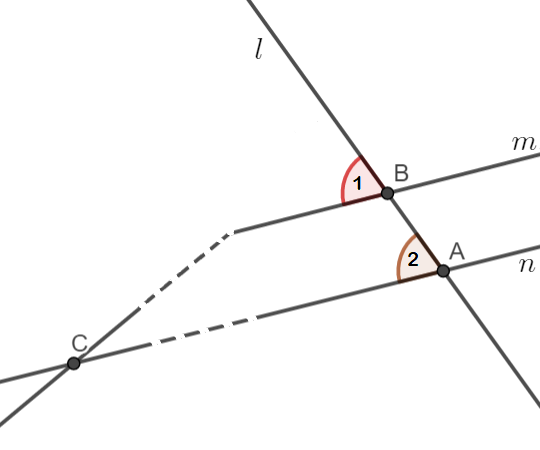
\includegraphics[width=0.27\textwidth]{tu/反证法1.png}
\end{wrapfigure}
当原命题是“任何”、“不存在”这种全判断的时候，它的否定是“至少有一个”这种有判断。这时，使用反证法就可以对这个“有一个”
的特例进行论证，非常方便。

\begin{tm}\label{tm:2-0-0}
    两条直线$m,n$交另一条直线$l$于两点。如果同位角相等，那么$m,n$平行。
\end{tm}
\begin{proof}
    使用反证法。命题“如果同位角相等，那么$m,n$平行”的否定是“有一对同位角相等，而且$m,n$不平行”。
    为了证明原命题是真的，我们假设它的否定是真的，然后推理得到矛盾。\\
    反设有一对同位角$\angle 1$和$\angle 2$相等，而且$m,n$不平行。设$m,n$的交点$C$在点$A$的一侧（如右图）。
    $\angle ACB + \angle 2$等于$\angle 1$的补角。但$\angle 1 = \angle 2$，
    所以$\angle ACB = 0^\circ$，这说明$m$和$n$重合而非平行。\\
    这就产生了矛盾！\\
    如果交点$C$在点$A$另一侧，通过类似推理可同样推出矛盾。\\
    这说明原命题的否定“有一对同位角相等，而且$m,n$不平行”是假的，因此原命题是真的。
\end{proof}

反证法的好处在于，通过假设命题的否定为真，我们多了一个用来推理的条件。

从定理\ref{tm:2-0-0}出发，可以证明它的逆命题。

\begin{tm}\label{tm:2-0-10}
    两条平行直线$m,n$交另一条直线$l$于两点，则同位角相等。
\end{tm}

\begin{proof}
    记$m,l$交点为$A$，$n,l$交点为$B$。
    过$B$作直线$n'$使得$n',l$的交角等于$m,l$的交角。由于这个交角就对应$m,n'$交$l$的同位角，
    所以根据定理\ref{tm:2-0-0}，$m,n'$平行。而根据平行公理，过直线外一点恰有一条直线与它平行。
    所以$n' = n$。这说明$m,n$交$l$的同位角相等。
\end{proof}

这里我们利用了平行公理的“唯一”性。这种利用“符合条件的恰有一个”来证明的方法称为\textbf{同一法}。

\begin{xt}
    \mbox{} \\
    \indent 1. 用反证法证明：如果任一整数$n$的立方是奇数，那么$n$也是奇数。\\
    \indent 2. 用反证法证明：所有奇数的平方除以$8$都余$1$。\\
    \indent 3. 用反证法证明垂距定理的逆命题：如果直线$l$外一点$P$到$l$上某点$Q$的距离不大于它到$l$上任何点的距离，
    那么$OQ \perp l$。\\
    \indent 4. 两条直线$m,n$交另一条直线$l$于两点。\\
    \indent 4.1. 用反证法证明：如果内侧角相等，那么$m,n$平行。\\
    \indent 4.1. 用反证法证明：如果同旁内角和为平角，那么$m,n$平行。\\
    动手做：\\
    \indent 补全定理\ref{tm:2-0-0}中根据“交点$C$在点$A$另一侧”推出矛盾的过程。
\end{xt}

\section{归纳法}
\begin{ex}\label{ex:2-2-0}
    观察并验证以下等式，你有什么发现？\\
    1. $1 + 3 = \frac12(3^2 - 1)$，$1 + 3 + 9 = \frac12(3^3 - 1)$，$1 + 3 + 9 + 27 = \frac12(3^4 - 1)$。\\
    2. $1 = \frac12(1+1)$，$1 + 2 = \frac22(1 + 2)$，$1 + 2 + 3 = \frac32(1 + 3)$。\\
    3. $\frac13 + \frac14 + \frac15 + \frac16 > \frac{9}{10}$，$\frac14 + \frac15 + \cdots + \frac{1}{9} > \frac{9}{10}$，
    $\frac15 + \frac16 + \cdots + \frac{1}{12} > \frac{9}{10}$。    
\end{ex}
从纷乱繁杂的事物中发现规律，是人类认识自然、改造自然的活动中不可缺少的一环。
归纳，就是试图用简单的规则概括已知的现象。比如，上面第一个例子中，我们可以归纳出这样的规律：
$$ \forall n \in \mathbb{N}, \,\,\, 1 + 3 + 3^2 + \cdots + 3^n = \frac{3^{n+1} - 1}{2}. $$
第二个例子中，我们可以归纳出：
$$ \forall n \in \mathbb{Z}^+, \,\,\, 1 + 2 + \cdots + n = \frac{n(n+1)}{2}. $$
第三个例子中，我们可以归纳出：
$$ \forall n \in \mathbb{Z}^+, \,\,\, \frac{1}{n+1} + \frac{1}{n+2} + \cdots + \frac{1}{3n} > \frac{9}{10}. $$
归纳得到的规律，并不总是正确的。比如，把$n=1$代入我们从第三个例子中归纳出来的不等式：
$$ \frac12 + \frac13 > \frac{9}{10}.$$
这个结论是错的。

怎样正确地归纳事物的规律呢？或者说，什么时候，我们可以确信归纳出的规律是正确的呢？
在漫长的数学研究中，人们认识到：
\begin{po}{\textbf{归纳公理}}
    设$P(n)$是一个含变量的命题，变量$n$可以是任意自然数。如果$P$满足以下两个条件：\\
    1. $P(0)$成立。\\
    2. 对每个自然数$n$，只要$P(n)$成立，$P(n+1)$就成立。\\
    那么，$P(n)$对任意自然数$n$都成立。
\end{po}
使用归纳公理的证明，也叫做用（数学）归纳法证明。用“数学”两个字，是为了和日常生活中凭有限经验归纳的做法区别开来。

以上三个例子中的规律，如何用归纳公理来论证呢？我们分别来写出过程。
\begin{proof}{\textbf{第一个例子 }}
    命题$P(n)$：
    $$ 1 + 3 + 3^2 + \cdots + 3^n = \frac{3^{n+1} - 1}{2}. $$
    按照归纳公理，要论证命题对任意自然数$n$都成立，我们分别验证两个条件：\\
    1. $P(0)$可以写成：$1 = \frac{3 - 1}{2}$，显然成立。\\
    2. 假设$P(n)$对某个自然数$n$成立，我们来证明$P(n+1)$成立。\\
    $P(n+1)$可以写成：
    $$ 1 + 3 + 3^2 + \cdots + 3^{n+1} = \frac{3^{n+2} - 1}{2}. $$
    由于$P(n)$成立，$(1)$式左边的前$n+1$项可以写成$\frac{3^{n+1} - 1}{2}$，于是两边同时减去这一项，得到：
    \begin{align*}
        3^{n+1} &= \frac{3^{n+2} - 1}{2} - \frac{3^{n+1} - 1}{2}  \\
        &= \frac{3\cdot 3^{n+1}}{2} - \frac{3^{n+1}}{2}  \\
        &= \frac{3\cdot 3^{n+1} - 3^{n+1}}{2}  \\
        &= \frac{2 \cdot 3^{n+1}}{2} = 3^{n+1} 
    \end{align*}
    显然成立。因此，根据归纳公理，$P(n)$对任意自然数$n$都成立。    
\end{proof}

我们可以看到，论证的时候，我们分别验证归纳公理要求的两个条件成立。从复杂的代数式到显然成立的等式，
我们用到了变量代换和因式分解的技巧。

\begin{proof}{\textbf{第二个例子 }}
    命题$P$只对正整数有定义，所以我们要证明$P(n)$对所有正整数$n$成立。
    为此，我们稍微改变一下论证方式。\\
    命题$P(n)$：
    $$ 1 + 2 + \cdots + n = \frac{n(n+1)}{2}. $$
    按照归纳公理，要论证命题对任意自然数$n$都成立，我们分别验证两个条件：\\
    1. $P(1)$可以写成：$1 = \frac{1(1+1)}{2}$，显然成立。\\
    2. 假设$P(n)$对某个自然数$n$成立，我们来证明$P(n+1)$成立。\\
    $P(n+1)$可以写成：
    $$ 1 + 2 + \cdots + (n+1) = \frac{(n+1)(n+2)}{2}.  $$
    由于$P(n)$成立，$(1)$式左边的前$n$项可以写成$\frac{n(n+1)}{2}$，于是两边同时减去这一项，得到：
    \begin{align*}
        n+1 &= \frac{(n+1)(n+2)}{2} - \frac{n(n+1)}{2}  \\
        &= \frac{n+1}{2}\left(n+2 - n\right)  \\
        &= \frac{n+1}{2} \cdot 2 = n+1 
    \end{align*}
    显然成立。因此，根据归纳公理，$P(n)$对任意正整数$n$都成立。    
\end{proof}

\begin{proof}{\textbf{第三个例子 }}
    命题$P(n)$：
    $$ \frac{1}{n+1} + \frac{1}{n+2} + \cdots + \frac{1}{3n} > \frac{9}{10}. $$
    我们已经验证过，$P(1)$不成立。现在利用归纳公理证明$P(n)$对大于等于$2$的自然数成立。
    为此，我们稍微改变一下论证方式。\\
    要论证命题对任意大于等于$2$的自然数$n$成立，我们分别验证两个条件：\\
    1. $P(2)$可以写成：
    $$\frac13 + \frac14 + \frac15 + \frac16 > \frac{9}{10}.$$
    计算可知等式左边等于$\frac{19}{20} > \frac{9}{10}$，因此$P(2)$成立。\\
    2. 假设$P(n)$对某个自然数$n$成立，我们来证明$P(n+1)$成立。\\
    $P(n+1)$可以写成：
    $$ \frac{1}{n+2} + \frac{1}{n+3} + \cdots + \frac{1}{3n+3} > \frac{9}{10}. $$
    由于$P(n)$成立，我们试着把上式左边用$P(n)$有关的式子表达出来，我们发现
    \begin{align*}
        \frac{1}{n+2} + \frac{1}{n+3} + \cdots + \frac{1}{3n+3} =& \frac{1}{n+1} + \frac{1}{n+2} + \cdots + \frac{1}{3n}  \\
        &+ \frac{1}{3n+1} + \frac{1}{3n+2} + \frac{1}{3n+3} - \frac{1}{n+1}  
    \end{align*}
    而
    \begin{align*}
        \frac{1}{3n+1} + \frac{1}{3n+2} + \frac{1}{3n+3} - \frac{1}{n+1} &>  \frac{1}{3n+3} + \frac{1}{3n+3} + \frac{1}{3n+3} - \frac{1}{n+1}  \\
        = \frac{3}{3n+3} - \frac{1}{n+1} = 0.  
    \end{align*}
    这说明：
    $$ \frac{1}{n+2} + \frac{1}{n+3} + \cdots + \frac{1}{3n+3} > \frac{1}{n+2} + \frac{1}{n+3} + \cdots + \frac{1}{3n}. $$
    $P(n)$告诉我们，上式右边大于$\frac{9}{10}$，所以上式左边也大于$\frac{9}{10}$。也就是说，$P(n+1)$成立。\\
    因此，根据归纳公理，$P(n)$对任意大于等于$2$的自然数$n$都成立。    
\end{proof}
从第二、第三个例子可以看出，归纳公理可以换个“开头”使用。为什么可以这么做呢？让我们来理解归纳公理是如何告诉我们$P(n)$对
任意自然数$n$都成立的。

举例来说，我们知道$P(0)$成立，并且只要$P(n)$成立，$P(n+1)$就成立。现在我们想知道$P(100)$为何成立。
论证过程是这样的：只要$P(n)$成立，$P(n+1)$就成立，而$P(0)$成立，所以$P(1)$也成立。接下来，既然$P(1)$成立，
我们又可以得到$P(2)$成立。以此类推，经过$100$次这样的推理，我们就知道，根据$P(99)$成立，有$P(100)$成立。

使用归纳公理，就好比跑步。第一个条件告诉我们从哪里出发；第二个条件告诉我们，可以一步一步跑下去。
第二、第三个例子的证明里，我们换了一个“起跑线”，但论证了每步都能接到下一步。
于是，我们可以从$1$或$2$出发，“跑”到每个大于等于$2$的自然数$n$那里去。

\begin{sk}\label{sk:2-2-1}
    想一想：\\
    小强在证明的时候用了这样的归纳法：\\
    首先证明：$P(0)$成立。然后证明：对每个自然数$n$，只要$P(1), P(2), \cdots , P(n)$成立，那么$P(n+1)$也成立。
    根据以上两点，就可以说命题$P(n)$对任意正整数成立。\\
    你觉得这个推理方法对吗？
\end{sk}

\section{无穷}
做整数除法的时候，我们会遇到两种情况：除得尽和除不尽。列出竖式后，我们用被除数减去除数和商的积，得到余数。
如果某次得到的余数是$0$，就说除法除得尽。如果每次余数都不是$0$，我们就说除法除不尽。举例来说，计算$4$除以$9$，
每步都用$4$加$0$得到$40$，减去$9\times 4=36$，再次得到$4$。我们可以不断按照竖式除法的规则做下去，
但这个过程是无穷无尽的。

夜晚，仰望星空的时候，我们说星星是数不尽的，星星离我们无限遥远。郊游时，看着满地的鲜花，我们说花儿是数不完的。
是因为星星和花朵的数量太多，数起来太费时间，还是因为它们不可能数得完？是因为星星和我们的距离太远，没有测量的办法，
还是因为它们不可能被测量出来？多、远、大、久这些概念，是否有尽头？我们日常形容多、远、大、久等概念的时候，会用“无限”、
“无穷”、“无尽”这样的词来修饰，以表达夸张。到底“无限”、“无穷”、“无尽”是什么意思呢？

为了好理解，我们用数数作为例子：从$1$开始数数，每次加$1$：$1,\,\,2,\,\,3,\cdots$。
会不会到了某一步，我们无法再数下去呢？

如果从$1$数到$1\dlim{0000}$，那么到了第$9999$步，我们就数完了。
如果从$1$数到$1000\dlim{0000}$，那么到了第$999\dlim{9999}$步，我们就数完了。

一般来说，如果要数的是前$n$个正整数，那么在第$n$步，我们就数完了，因为$n+1$乃至更大的数都不在前$n$个正整数里。

但是，如果要数的是全体正整数，那么我们可以一直数下去。因为每个正整数$n$后面的数：$n+1$都是正整数。
所以，全体正整数集合和前$1\dlim{0000}$个正整数、前$1000\dlim{0000}$个正整数或前$n$个正整数构成的集合不一样。

数学中，我们可以将集合分为两类。一类称为\textbf{有限}或\textbf{有穷}，一类称为\textbf{无限}或\textbf{无穷}。
前$1\dlim{0000}$个正整数、前$1000\dlim{0000}$个正整数、前$n$个正整数这样的集合是有限或有穷的。
全体正整数、全体自然数这样的集合是无限或无穷的。

我们把前面“数数”的方法推广到一般的集合，判别集合有穷还是无穷。
一开始，集合所有的元素都是没数过的。
我们逐个来数它的元素：每次选择一个没数过的元素，
把它标记为数过的。这样，就说这个元素被数到了。
每个元素至多被数到一次，从没数过的元素变成数过的元素。

如果无论每次依什么规则选取元素，
数数过程都会因为没有没数过的数而停止，就说集合是有穷的，或集合元素的个数是有穷的。如果依照某个规则，数数过程不会停止，
就说集合是无穷的，或集合元素的个数是无穷的。

概括来说，数得尽的集合是有穷的，数不尽的集合是无穷的。我们把这种判别方法称为\textbf{数数原则}。

前面我们给正整数设计的数数规则就是一种不会停止的规则：选择上次数到的数加$1$得到的数。一方面，按照这个规则，
每次数到的数总是数过的数里最大的。另一方面，正整数加$1$总是正整数，所以按照规则，
用上次数到的数加$1$，就得到一个没数过的正整数。
按照数数原则，我们可以判定：全体正整数是无穷的。

依照同一个规则，我们也可以判定：全体自然数是无穷的。

对于前$n$个自然数的集合，我们可以证明它是有穷的。

记前$n$个自然数的集合为$X_n$，数数过程中，记第$i$步结束后所有没数过的数的个数为$G(i)$。
记一开始所有没数过的数的个数为$G(0)$，则$G(0) = n$。无论用什么规则，每一步结束后，没数过的数都少了一个，
即$G(i+1) = G(i) - 1$。于是，$G(n) = G(0) - n = 0$。第$n$步后，不再有没数过的数，数数过程只能停止。
根据数数原则，$X_n$是有穷的。

要注意的是，数数原则并不总要求每个数都被数过。如果集合是有穷的，按照定义，停止时所有的数都被数过了；
如果集合是无穷的，那么由于数数过程不会停止，不一定每个数都被数过。
比如，我们按照每次加$2$的方式给全体正整数的集合数数：
$1,3,5,\cdots$。这个过程不会停止，但偶数永远不会被数到。

\begin{sk}
    \mbox{}\\
    \indent 1. “除不尽”的例子中，什么是无穷的？\\
    \indent 2. 全体偶数是否是无穷的？全体整数是否是无穷的？全体有理数呢？你可以总结出什么规律？
\end{sk}
